\documentclass[dvipdfmx, 9pt, a4paper]{article}
\usepackage[margin=15mm]{geometry}
\usepackage{fancyhdr}
\usepackage{multirow}
\usepackage{amsmath,  amssymb}
\usepackage{type1cm}
\usepackage{latexsym}
\usepackage{algorithmic}
\usepackage{algorithm}
\usepackage{ascmac}
\usepackage{listings,jvlisting}
\usepackage{tcolorbox}
\usepackage[utf8]{inputenc}
\usepackage{color}

\DeclareFixedFont{\ttb}{T1}{txtt}{bx}{n}{9}
\DeclareFixedFont{\ttm}{T1}{txtt}{m}{n}{9}
\definecolor{deepblue}{rgb}{0,0,0.5}
\definecolor{deepred}{rgb}{0.6,0,0}
\definecolor{deepgreen}{rgb}{0,0.5,0}

\renewcommand{\theequation}{\arabic{section}.\arabic{equation}}
\renewcommand{\thefigure}{\arabic{section}.\arabic{figure}}
\renewcommand{\thetable}{\arabic{section}.\arabic{table}}
\makeatletter
\@addtoreset{equation}{section}
\@addtoreset{figure}{section}
\@addtoreset{table}{section}
\AtBeginDocument{
  \renewcommand*{\thelstlisting}{\arabic{section}.\arabic{lstlisting}}%
  \@addtoreset{lstlisting}{section}
}

\numberwithin{equation}{section}

\renewcommand{\baselinestretch}{0.78}
\newcommand{\bm}[1]{{\mbox{\boldmath $#1$}}}
\newcommand{\bnabla}{\bm \nabla}
\newtheorem{Proof}{証明}
\def\qed{\hfill $\Box$}

\lstset{%language=Fortran,%
        basicstyle=\footnotesize,%
        commentstyle=\textit,%
        classoffset=1,%
        keywordstyle=\bfseries,%
	frame=tRBl,framesep=5pt,%
	showstringspaces=false,%
        numbers=left,stepnumber=1,numberstyle=\footnotesize%
	}%


\begin{document}
\begin{center}
{\fontsize{18pt}{1pt}\selectfont Gmsh}\\
\end{center}
\section{Overview of Gmsh}
Gmsh is a three-dimensional finite element mesh generator with a build-in CAD engine and post-processor. Its design goal is to provide a fast, light and user-friendly meshing tool with parametric input and flexible visualization capabilities.\par
Gmsh is built around four modules (geometry, mesh, solver and post-processing), which can be controlled with the graphical user interface,  from the command line, using text files written in Gmsh's own scripting language, or through the C++, C, Python, Julia and Fortran application programming interface\par
A brief description of the four modules is given hereafter, before an overview of what Gmsh does best (... and what it is not so good at), and some practical information on how to install and run Gmsh on your computer.

\subsection{Geometry module}
A model in Gmsh is defined using its Boundary Representation (BRep): a volume is bounded by a set of surfaces, a surface is bounded by a series of curves, and a curve is bounded by two end points. Model entities are topological entities, i.e., they only deal with adjacencies in the model, and are implemented as a set of abstract topological classes. This BRep is extended by the definition of embedded, or internal, model entities: internal points, curves and surfaces can be embedded in volumes; and internal points and curves can be embedded in surfaces. \par
The geometry of model entities can be provided by different CAD kernels. The two default kernels interfaced by Gmsh are the built-in kernel and the OpenCASCADE kernel. Gmsh does not translate the geometrical representation from one kernel to another, or from these kernels to some neutral representation. Instead, Gmsh directly queries the native data for each CAD kernel, which avoids data loss and is crucial for complex models where translations invariably introduce issues linked to slightly different representations.  Selecting the CAD kernel in `.geo` scripts is done with the SetFactory command, while in the Gmsh API the kernel appears explicitly in all the relevant functions from the gmsh/model namespace, with geo or occ prefixes for the built-in and OpenCASCADE kernel, respectively.\par
Entities can either be built in a bottom-up manner (first points, then curves, surfaces and volumes) with the built-in and OpenCASCADE kernels, or in a top-down constructive solid geometry fashion (solids on which boolean operations are performed) with the OpenCASCADE kernel. Both methodologies can also be combined. Finally, groups of model entities (called "physical groups") can be defined, based on the elementary geometric entities.\par
Both model entities (also referred to as "elementary entities") and physical groups are uniquely defined by a pair of integers: their dimension (0 for points, 1 for curves, 2 for surfaces, 3 for volumes) and their tag, a strictly positive global identification number. Entity and group tags are unique per dimension:
\begin{enumerate}
\item  each point must possess a unique tag
\item  each point curve possess a unique tag
\item  each point surface possess a unique tag
\item  each point volume possess a unique tag
\end{enumerate}
Zero or negative tags are reserved by Gmsh for internal use.\par
Model entities can be manipulated and transformed in a variety of ways within the geometry module, but operations are always performed directly within their respective CAD kernels. As explained above, there is no common internal geometrical representation: rather, Gmsh directly performs the operations (translation, rotation, intersection, union, fragments, ...) on the native geometrical representation using each CAD kernel's own API. In the same philosophy, models can be imported in the geometry module through each CAD kernel's own import mechanisms. For example, by default Gmsh imports STEP and IGES files through OpenCASCADE, which will lead to the creation of model entities with an internal OpenCASCADE representation.\par
The Chapter 2 is the best place to learn how to use the geometry module: it contains examples of increasing complexity based on both the built-in and the OpenCASCADE kernel. Note that many features of the geometry module can be used interactively in the GUI, which is also a good way to learn about both Gmsh's scripting language and the API, as actions in the geometry module automatically append the related command in the input script file, and can optionally also generate input for the languages supported by the API (see the General.ScriptingLanguages option; this is still work-in-progress as of Gmsh 4.12.)\par
In addition to CAD-type geometrical entities, whose geometry is provided by a CAD kernel, Gmsh also supports discrete model entities, which are defined by a mesh (e.g. STL). Gmsh does not perform geometrical operations on such discrete entities, but they can be equipped with a geometry through a so-called "reparametrization" procedure. The parametrization is then used for meshing, in exactly the same way as for CAD entities.
\subsection{Mesh module}
A finite element mesh of a model is a tessellation of its geometry by simple geometrical elements of various shapes (in Gmsh: lines, triangles, quadrangles, tetrahedra, prisms, hexahedra and pyramids), arranged in such a way that if two of them intersect, they do so along a face, an edge or a node, and never otherwise. This defines a so-called conformal mesh. The mesh module implements several algorithms to generate such meshes automatically. By default, meshes produced by Gmsh are considered as unstructured, even if they were generated in a structured way (e.g., by extrusion). This implies that the mesh elements are completely defined simply by an ordered list of their nodes, and that no predefined ordering relation is assumed between any two elements.\par
In order to guarantee the conformity of the mesh, mesh generation is performed in a bottom-up flow: curves are discretized first; the mesh of the curves is then used to mesh the surfaces; then the mesh of the surfaces is used to mesh the volumes. In this process, the mesh of an entity is only constrained by the mesh of its boundary, unless entities of lower dimensions are explicitly embedded in entities of higher dimension. For example, in three dimensions, the triangles discretizing a surface will be forced to be faces of tetrahedra in the final 3D mesh only if the surface is part of the boundary of a volume, or if that surface has been explicitly embedded in the volume. This automatically ensures the conformity of the mesh when, for example, two volumes share a common surface. Mesh elements are oriented according to the geometrical orientation of the underlying entity. Every meshing step is constrained by a mesh size field, which prescribes
the desired size of the elements in the mesh. This size field can be uniform, specified by values associated with points in the geometry, or defined by general mesh size fields (for example related to the distance to some boundary, to a arbitrary scalar field defined on another mesh, etc.).  For each meshing step, all structured mesh directives are executed first, and serve as additional constraints for the unstructured parts.(The generation and handling of conformal meshes has important consequences on how meshes are stored internally in Gmsh, and how they are accessed through the API)\par
Gmsh's mesh module regroups several 1D, 2D and 3D meshing algorithms:
\begin{itemize}
\item The 2D unstructured algorithms generate triangles and/or quadrangles (when recombination commands or options are used). The 3D unstructured algorithms generate tetrahedra, or tetrahedra and pyramids (when the boundary mesh contains quadrangles).
\item The 2D structured algorithms (transfinite and extrusion) generate triangles by default, but quadrangles can be obtained by using the recombination commands or options. The 3D structured algorithms generate tetrahedra, hexahedra, prisms and pyramids, depending on the type of the surface meshes they are based on.
\end{itemize}
All meshes can be subdivided to generate fully quadrangular or fully hexahedral meshes with the Mesh.SubdivisionAlgorithm option.
\subsubsection{Choosing the right unstructured algorithm}
Gmsh provides a choice between several 2D and 3D unstructured algorithms. Each algorithm has its own advantages and disadvantages.\par
For all 2D unstructured algorithms a Delaunay mesh that contains all the points of the 1D mesh is initially constructed using a divide-and-conquer algorithm. Missing edges are recovered using edge swaps. After this initial step several algorithms can be applied to generate the final mesh:
\begin{itemize}
\item The "MeshAdapt" algorithm is based on local mesh modifications. This technique makes use of edge swaps, splits, and collapses: long edges are split, short edges are collapsed, and edges are swapped if a better geometrical configuration is obtained.
\item The "Delaunay" algorithm is inspired by the work of the GAMMA team at INRIA. New points are inserted sequentially at the circumcenter of the element that has the largest adimensional circumradius. The mesh is then reconnected using an anisotropic Delaunay
criterion.
\item The "Frontal-Delaunay" algorithm is inspired by the work of S. Rebay.
\item Other experimental algorithms with specific features are also available. In particular, "Frontal-Delaunay for Quads" is a variant of the "Frontal-Delaunay" algorithm aiming at generating right-angle triangles suitable for recombination; and "BAMG" allows to generate anisotropic triangulations.
\end{itemize}
For very complex curved surfaces the "MeshAdapt" algorithm is the most robust. When high element quality is important, the "Frontal-Delaunay" algorithm should be tried. For very large meshes of plane surfaces the "Delaunay" algorithm is the fastest; it usually also handles complex mesh size fields better than the "Frontal-Delaunay"  When the "Delaunay" or "Frontal Delaunay" algorithms fail, "MeshAdapt" is automatically triggered. The "Automatic" algorithm uses "Delaunay" for plane surfaces and "MeshAdapt" for all other surfaces.\par
Several 3D unstructured algorithms are also available:
\begin{itemize}
\item The "Delaunay" algorithm is split into three separate steps. First, an initial mesh of the union of all the volumes in the model is performed, without inserting points in the volume. The surface mesh is then recovered using H. Si's boundary recovery algorithm Tetgen/BR. Then a three-dimensional version of the 2D Delaunay algorithm described above is applied to insert points in the volume to respect the mesh size constraints.
\item The "Frontal" algorithm uses J. Schoeberl's Netgen algorithm.
\item The "HXT" algorithm is a new efficient and parallel reimplementaton of the Delaunay algorithm.
\item Other experimental algorithms with specific features are also available. In particular, "MMG3D" allows to generate anisotropic tetrahedralizations.
\end{itemize}
The "Delaunay" algorithm is currently the most robust and is the only one that supports the automatic generation of hybrid meshes with pyramids. Embedded model entities and general mesh size fields are currently only supported by the "Delaunay" and "HXT" algorithms.\par
When Gmsh is configured with OpenMP support, most of the meshing steps can be performed in parallel:
\begin{itemize}
\item 1D and 2D meshing is parallelized using a coarse-grained approach, i.e. curves (resp. surfaces) are each meshed sequentially, but several curves (resp. surfaces) can be meshed at the same time.
\item 3D meshing using HXT is parallelized using a fine-grained approach, i.e. the actual meshing procedure for a single volume is done is parallel.
\end{itemize}
The number of threads can be controlled with the -nt flag on the command lin, or with the General.NumThreads, Mesh.MaxNumThreads1D, Mesh.MaxNumThreads2D and Mesh.MaxNumThreads3D options.
\subsubsection{Specifying mesh element sizes}
There are several ways to specify the size of the mesh elements for a given geometry:
\begin{enumerate}
\item First, if the options Mesh.MeshSizeFromPoints and Mesh.MeshSizeExtendFromBoundary are set, you can simply specify desired mesh element sizes at the geometrical points of the model. The size of the mesh elements will then be computed by interpolating these values inside the domain during mesh generation. This might sometimes lead to over-refinement in some areas, so that you may have to add "dummy" geometrical entities in the model in order to get the desired element sizes or use more advanced methods explained below.
\item  Second, if Mesh.MeshSizeFromCurvature is set to a positive value (it is set to 0 by default), the mesh will be adapted with respect to the curvature of the model entities, the value giving the target number of elements per 2 Pi radians.
\item Next, you can specify a general target mesh size, expressed as a combination of mesh size fields:
\begin{itemize}
\item The Box field specifies the size of the elements inside and outside of a parallelepipedic region.
\item The Distance field specifies the size of the mesh according to the distance to some model entities.
\item The MathEval field specifies the size of the mesh using an explicit mathematical function.
\item The PostView field specifies an explicit background mesh in the form of a scalar post processing view in which the nodal values are the target element sizes. This method is very general but it requires a first (usually rough) mesh and a way to compute the target sizes on this mesh (usually through an error estimation procedure, e.g. in an iterative process of mesh adaptation).
\item The Min field specifies the size as the minimum of the sizes computed using other fields
\item ...
\end{itemize}
\item Mesh sizes are also constrained by structured meshing constraints (e.g. transfinite or extruded meshes) as well as by any discrete model entity that is not equipped with a geometry, and which will thus preserve it mesh during mesh generation.
\item Boundary mesh sizes are interpolated inside surfaces and/or volumes depending on the value of\\ Mesh.MeshSizeExtendFromBoundary.
\end{enumerate}
To determine the actual mesh size at any given point in the model, Gmsh evaluates all the above mesh size constraints and selects the smallest value. Using the Gmsh API, this value can then be further modified using a C++, C, Python, Julia or Fortran mesh size callback function provided via gmsh/model/mesh/setSizeCallback.\par
The resulting value is further constrained in the interval [ Mesh.MeshSizeMin, Mesh.MeshSizeMax ] (which can also be provided on the command line with -clmin and -clmax). The resulting value is then finally multiplied by Mesh.MeshSizeFactor (-clscale on the command line).\par
Note that when the element size is fully specified by a mesh size field, it is thus often desirable to set
\begin{lstlisting}
Mesh.MeshSizeFromPoints = 0;
Mesh.MeshSizeFromCurvature = 0;
Mesh.MeshSizeExtendFromBoundary = 0;
\end{lstlisting}
to prevent over-refinement inside an entity due to small mesh sizes on its boundary.

\subsubsection{Elementary entities vs. physical groups}
It is usually convenient to combine elementary geometrical entities into more meaningful groups, e.g. to define some mathematical ("domain", "boundary with Neumann condition"), functional ("left wing", "fuselage") or material ("steel", "carbon") properties. Such grouping is done in Gmsh's geometry module through the definition of "physical groups".\par
By default in the native Gmsh MSH mesh file format, as well as in most other mesh formats, if physical groups are defined, the output
mesh only contains those elements that belong to at least one physical group. (Different mesh file formats treat physical groups in slightly different ways, depending on their capability to define groups.) To save all mesh elements whether or not physical groups are defined, use the Mesh.SaveAll option or specify -save\_all on the command line. In some formats (e.g. MSH2), setting Mesh.SaveAll will however discard all physical group definitions.

\subsection{Solver module}
Gmsh implements a ONELAB server to exchange data with external solvers or other codes (called "clients"). The ONELAB interface allows to call such clients and have them share parameters and modeling information.\par
The implementation is based on a client-server model, with a server-side database and local or remote clients communicating in-memory or through TCP/IP sockets. Contrary to most solver interfaces, the ONELAB server has no a priori knowledge about any specifics (input file format, syntax, ...) of the clients. This is made possible by having any simulation preceded by an analysis phase, during which the clients are asked to upload their parameter set to the server. The issues of completeness and consistency of the parameter sets are completely dealt with on the client side: the role of ONELAB is limited to data centralization, modification and re-dispatching.
Using the Gmsh API, you can directly embed Gmsh in your C++, C, Python, Julia or Fortran solver, use ONELAB for interactive parameter definition and modification, and to create post processing data on the fly. See prepro.py, custom gui.py and custom gui.cpp for examples. If you prefer to keep codes separate, you can also communicate with Gmsh through a socket by providing the solver name (Solver.Name0, Solver.Name1, etc.) and the path to the executable (Solver.Executable0, Solver.Executable1, etc.). Parameters can then be exchanged using the ONELAB protocol: see the utils/solvers directory for examples. A full-featured solver interfaced in this manner is GetDP, a general finite element solver using mixed finite elements.

\subsection{Post-processing module}
The post-processing module can handle multiple scalar, vector or tensor datasets along with the geometry and the mesh. The datasets can be given in several formats: in human-readable "parsed" format (these are just part of a standard input script, but are usually put in separate files with a '.pos' extension), in native MSH files (ASCII or binary files with '.msh' extensions), or in standard third-party formats such as CGNS or MED. Datasets can also be directly imported using the Gmsh API. Once loaded into Gmsh, scalar fields can be displayed as iso-curves, iso-surfaces or color maps, whereas vector fields can be represented either by three-dimensional arrows or by displacement maps. Tensor fields can be displayed as Von-Mises effective stresses, min/max eigenvalues, eigenvectors, ellipses or ellipsoids. (To display other combinations of components, you can use the View.ForceNumComponents option. Each dataset, along with the visualization options, is called a "post-processing view", or simply a "view". Each view is given a name, and can be manipulated either individually (each view has its own button in the GUI and can be referred to by its index or its unique tag in a script or in the API) or globally. Possible operations on post-processing views include section computation, offset, elevation, boundary and component extraction, color map and range modification, animation, vector graphic output, etc. These operations are either carried out nondestructively through
the modification of post-processing options, or can lead to the actual modification of the view data or the creation of new views when done using post-processing plugins. Both can be fully automated in scripts or through the API.\par
By default, Gmsh treats all post-processing views as three-dimensional plots, i.e., draws the scalar, vector and tensor primitives (points, curves, triangles, tetrahedra, etc.) in 3D space. But Gmsh can also represent each post-processing view containing scalar points as two-dimensional ("X-Y") plots, either space- or time-oriented:
\begin{itemize}
\item in a '2D space' plot, the scalar points are taken in the same order as they are defined in the post-processing view: the abscissa of the 2D graph is the curvilinear abscissa of the curve defined by the point series, and only one curve is drawn using the values associated with the points. If several time steps are available, each time step generates a new curve;
\item in a '2D time' plot, one curve is drawn for each scalar point in the view and the abscissa is the time step.
\end{itemize}
\section{Gmsh scrpiting language}
The Gmsh scripting language is interpreted at runtime by Gmsh's parser. Scripts are written in ASCII files and are usually given the '.geo' extension, but any extension (or no extension at all) can also be used. For example Gmsh often uses the '.pos' extension for scripts that
contain post-processing commands, in particular parsed post-processing views.\par
Historically, '.geo' scripts have been the primary way to perform complex tasks with Gmsh, and they are indeed quite powerful: they can handle (lists of) floating point and string variables, loops and tests, macros, etc. However Gmsh's scripting language is still quite limited compared to actual programming languages: for example there are no private variables, macros don't take arguments, and the runtime interpretation by the parser can penalize performance on large models. Depending on the workflow and the application, using the Gmsh API can thus sometimes be preferable. The downside of the API is that, while the scripting language is baked into Gmsh and is thus available directly in the standalone Gmsh app, the API requires external dependencies (a C++, C or Fortran compiler; or a Python or Julia interpreter).\par
This chapter describes the scripting language by detailing general commands first, before detailing the scripting commands specific to the
geometry, mesh and post-processing modules.\par
The following rules are used when describing the scripting language in the rest of this chapter (note that metasyntactic variable definitions stay valid throughout the chapter, not only in the section where the definitions appear):
\begin{enumerate}
\item Keywords and literal symbols are printed like {\bf this}.
\item Metasyntactic variables (i.e., text bits that are not part of the syntax, but stand for other text bits) are printed like {\it this}.
\item A colon (:) after a metasyntactic variable separates the variable from its definition.
\item Optional rules are enclosed in $< >$ pairs.
\item  Multiple choices are separated by $|$.
\item Three dots (. . . ) indicate a possible (multiple) repetition of the preceding rule.
\end{enumerate}

\subsection{General scripting commands}
\subsubsection{Comments}
Gmsh script files support both C and C++ style comments:
\begin{enumerate}
\item any text comprised between /* and */ pairs is ignored;
\item the rest of a line after a double slash // is ignored.
\end{enumerate}
These commands won't have the described effects inside double quotes or inside keywords. Also note that white space (spaces, tabs, new line characters) is ignored inside all expressions.
\subsubsection{Floating point expression}
The two constant types used in Gmsh scripts are real and string (there is no integer type). These types have the same meaning and syntax as in the C or C++ programming languages.\par
Floating point expressions (or, more simply, expressions) are denoted by the metasyntactic variable expression, and are evaluated during the parsing of the script file:
\begin{itemize}
\item {\it expression} :
\begin{itemize}
\item {\it real}
\item {\it string}
\item {\it string}\textasciitilde\{ {\it expression} \}
\item {\it string} [ expression ]
\item \# {\it string} [ ]
\item ( {\it expression} )
\item {\it operator-unary-left expression}
\item {\it operator-unary-right expression}
\item {\it operator-binary expression}
\item {\it operator-ternary-left expression operator-ternary-right expression}
\item {\it built-in-function}
\item {\it number-option}
\item Find({\it expression-list-item, expression-list-item})
\item StrFind({\it string-expression, string-expression})
\item StrFind({\it string-expression, string-expression})
\item StrCmp({\it string-expression, string-expression})
\item StrLen({\it string-expression})
\item TextAttributes({\it string-expression$<$, string-expression...$>$})
\item Exists({\it string})
\item Exists({\it string}\textasciitilde\{ {\it expression} \})
\item FileExists({\it string-expression})
\item StringToName({\it string-expression})
\item S2N({\it string-expression})
\item GetNumber({\it string-expression $<$, expression$>$})
\item GetValue({\it "string", expression})
\item DefineNumber({\it expression, onelab-options})
\end{itemize}
\end{itemize}
Such expressions are used in most of Gmsh's scripting commands. When \textasciitilde\{expression\} is appended to a string string, the result is a new string formed by the concatenation of string, \_(an underscore) and the value of the expression. This is most useful in loops, where it permits to define unique strings automatically. Forexample,
\begin{lstlisting}
For i In {1:3}
    x~{i} = i;
EndFor
\end{lstlisting}
is the same as
\begin{lstlisting}
x_1 = 1;
x_2 = 2;
x_3 = 3;
\end{lstlisting}
The brackets [ ] permit to extract one item from a list (parentheses can also be used instead of brackets). The \# permits to get the size of a list. Find searches for occurrences of the first expression in the second (both of which can be lists). StrFind searches the first string-expression for any occurrence of the second string-expression. StrCmp compares the two strings (returns an integer greater than, equal to, or less than 0, according as the first string is greater than, equal to, or less than the second string). StrLen returns the length of the string. TextAttributes creates attributes for text strings. Exists checks if a variable with the given name exists (i.e., has been defined previously), and FileExists checks if the file with the given name exists. StringToName creates a name from the provided string. GetNumber allows to get the value of a ONELAB variable (the optional second argument is the default value returned if the variable does not exist). GetValue allows to ask the user for a value interactively (the second argument is the value returned in non-interactive mode). For example, inserting GetValue("Value of parameter alpha?", 5.76) in an input file will query the user for the value of a certain parameter alpha, assuming the default value is 5.76. If the option General.NoPopup is set, no question is asked and the default value is automatically used.\par
DefineNumber allows to define a ONELAB variable in-line. The expression given as the first argument is the default value; this is followed by the various ONELAB options. See the ONELAB tutorial wiki for more information.\par
List of expressions are also widely used, and are defined as:
\begin{itemize}
\item {\it expression-list} : {\it expression-list-item $<$, expression-list-item$>$ ...}
\end{itemize}
with
\begin{itemize}
\item {\it expression-list-item}
\begin{itemize}
\item {\it expression}
\item {\it expression : expression}
\item {\it expression : expression : expression}
\item {\it string} [ ]
\item {\it string} ()
\item List [{\it string}]
\item List [{\it expression-list-item }]
\item List [\{ {\it expression-list } \}]
\item Unique [{\it expression-list-item} ]
\item ListFromFile [{\it expression-char}]
\item LinSpace [{\it expression : expression : expression}]
\item LogSpace [{\it expression : expression : expression}]
\item {\it string} [\{ {\it expression-list} \}]
\item Point \{ {\it expression} \}
\item {\it transform}
\item {\it extrude}
\item {\it boolean}
\item Point$|$Curve$|$Surface$|$Volume In BoundingBox \{ {\it expression-list }\}
\item BoundingBox Point$|$Curve$|$Surface$|$Volume \{ {\it expression-list } \}
\item Mass Curve$|$Surface$|$Volume \{{\it expression} \}
\item CenterOfMass Curve$|$Surface$|$Volume \{ {\it expression } \}
\item MatrixOfInertia Curve$|$Surface$|$Volume \{ {\it expression }\}
\item Point \{{\it expression }\}
\item Physical Point$|$Curve$|$Surface$|$Volume \{{\it expression-list }\}
\item $<$Physical$>$ Point$|$Curve$|$Surface$|$Volume \{ : \}
\end{itemize}
\end{itemize}
The second case in this last definition permits to create a list containing the range of numbers comprised between two expressions, with a unit incrementation step. The third case also permits to create a list containing the range of numbers comprised between two expressions, but with a positive or negative incrementation step equal to the third expression. The fourth, fifth and sixth cases permit to reference an expression list (parentheses can also be used instead of brackets). Unique sorts the entries in the list and removes all duplicates. Abs takes the absolute value of all entries in the list. ListFromFile reads a list of numbers from a file. LinSpace and LogSpace construct lists using linear or logarithmic spacing. The next two cases permit to reference an expression sublist (whose elements are those corresponding to the indices provided by the expression-list). The next cases permit to retrieve the indices of entities created through geometrical transformations, extrusions and boolean operations.\par
The next two cases allow to retrieve entities in a given bounding box, or get the bounding box of a given entity, with the bounding box specified as (X min, Y min, Z min, X max, Y max, Z max). Beware that the order of coordinates is different than in the BoundingBox command for the scene. The last cases permit to retrieve the mass, the center of mass or the matrix of inertia of an entity, the coordinates of a given geometry point, the elementary entities making up physical groups, and the tags of all (physical or elementary) points, curves, surfaces or volumes in the model. These operations all trigger a synchronization of the CAD model with the internal Gmsh model.\par
For some commands it makes sense to specify all the possible expressions in a list. This is achieved with expression-list-or-all, defined as:
\begin{itemize}
\item {\it expression-list-or-all} :
\begin{itemize}
\item {\it expression-list} $|$ :
\end{itemize}
\end{itemize}
The meaning of "all"(:) depends on context. For example, Curve \{ : \} will get the ids of all the existing curves in the model, while Surface \{ : \} will get the ids of all existing surfaces.
\subsubsection{String expressions}
String expressions are defined as:
\begin{itemize}
\item {\it string-expression}
\begin{itemize}
\item "{\it string}"
\item {\it string}
\item {\it string} [ {\it expression} ]
\item Today
\item OnelabAction
\item GmshExecutableName
\item CurrentDirectory $|$ CurrentDir $|$ CurrentFileName
\item StrPrefix ( {\it string-expression} )
\item StrRelative ( {\it string-expression} )
\item StrCat ( {\it string-expression} $<$,...$>$ )
\item Str ( {\it string-expression} $<$,...$>$ )
\item StrChoice ( {\it expression, string-expression, string-expression} )
\item StrSub( {\it string-expression, expression, expression} )
\item StrSub( {\it string-expression, expression} )
\item UpperCase ( {\it string-expression} )
\item AbsolutePath ( {\it string-expression} )
\item DirName ( {\it string-expression} )
\item Sprintf ( {\it string-expression , expression-list} )
\item Sprintf ( {\it string-expression} )
\item Sprintf ( {\it string-option} )
\item GetEnv ( {\it string-expression} )
\item GetString ( {\it string-expression $<$,string-expression$>$})
\item GetStringValue ( {\it string-expression , string-expression} )
\item StrReplace ( {\it string-expression , string-expression , string-expression} )
\item NameToString ( {\it string} )
\item N2S ( {\it string} )
\item $<$Physical$>$ Point$|$Curve$|$Surface$|$Volume \{ {\it expression }\}
\item DefineString({\it string-expression, onelab-options})
\end{itemize}
\end{itemize}
Today returns the current date. OnelabAction returns the current ONELAB action (e.g. check or compute). GmshExecutableName returns the full path of the Gmsh executable. CurrentDirectory (or CurrentDir) and CurrentFileName return the directory and file name of the script being parsed. StrPrefix and StrRelative take the prefix (e.g. to remove the extension) or the relative path of a given file name. StrCat and Str concatenate string expressions (Str adds a newline character after each string except the last). StrChoice returns the first or second string-expression depending on the value of expression. StrSub returns the portion of the string that starts at the character position given by the first expression and spans the number of characters given by the second expression or until the end of the string (whichever comes first; or always if the second expression is not provided). UpperCase converts the string expression to upper case. AbsolutePath returns the absolute path of a file. DirName returns the directory of a file. Sprintf is equivalent to the sprintf C function (where string-expression is a format string that can contain floating point formatting characters: \%e, \%g, etc.) GetEnvThe gets the value of an environment variable from the operating system. GetString allows to get a ONELAB string value (the second optional argument is the default value returned if the variable does not exist). GetStringValue asks the user for a value interactively (the second argument is the value used in non-interactive mode). StrReplace's arguments are: input string, old substring, new substring (brackets can be used instead of parentheses in Str and Sprintf). Physical Point, etc., or Point, etc., retrieve the name of the physical or elementary entity, if any. NameToString converts a variable name into a string.\par
DefineString allows to define a ONELAB variable in-line. The string-expression given as the first argument is the default value; this is followed by the various ONELAB options. See the ONELAB tutorial wiki for more information.\par
String expressions are mostly used to specify non-numeric options and input/output file names.\par
List of string expressions are defined as:
\begin{itemize}
\item {\it string-expression-list} :
\begin{itemize}
\item {\it string-expression} $<, ...>$
\end{itemize}
\end{itemize}

\subsubsection{Color expressions}
Colors expressions are hybrids between fixed-length braced expression-lists and strings:
\begin{itemize}
\item {\it color-expression} : 
\begin{itemize}
\item {\it string-expression}
\item \{{\it expression, expression, expression} \}
\item \{{\it expression, expression, expression, expression} \}
\item {\it color-option}
\end{itemize}
\end{itemize}
The first case permits to use the X Windows names to refer to colors, e.g., Red, SpringGreen, LavenderBlush3, . . . (see src/common/Colors.h in the source code for a complete list). The second case permits to define colors by using three expressions to specify their red, green and blue components (with values comprised between 0 and 255). The third case permits to define colors by using their red, green and blue color components as well as their alpha channel. The last case permits to use the value of a color-option as a color-expression.

\subsubsection{Operators}
Gmsh's operators are similar to the corresponding operators in C and C++. Here is the list of available unary, binary and ternary operators.
\begin{itemize}
\item operator-unary-right
\begin{itemize}
\item - : Unary minus.
\item ! : Logical not.
\end{itemize}
\item operator-unary-right:
\begin{itemize}
\item ++ : Post-incrementation.
\item -- : Post-decrementation.
\end{itemize}
\item  operator-binary:
\begin{itemize}
\item \^{} : Exponentiation.
\item * : Multiplication.
\item / : Division.
\item \% : Modulo.
\item + : Addition.
\item - : Subtraction.
\item == : Equality.
\item != : Inequality.
\item $>$ : Greater.
\item $>=$ : Greater or equality.
\item $<$ : Less.
\item $<=$ : Less or equality.
\item \&\& : Logical ‘and’.
\item $||$ : Logical 'or'. (Warning: the logical 'or' always implies the evaluation of both arguments. That is, unlike in C or C++, the second operand of || is evaluated even if the first one is true).
\end{itemize}
\item operator-ternary-left
\begin{itemize}
\item ?
\end{itemize}
\item operator-ternary-right
\begin{itemize}
\item : : The only ternary operator, formed by operator-ternary-left and operator-ternary-right, returns the value of its second argument if the first argument is non-zero; otherwise it returns the value of its third argument.
\end{itemize}
\end{itemize}
The evaluation priorities are summarized below (from stronger to weaker, i.e., * has a highest evaluation priority than +). Parentheses () may be used anywhere to change the order of evaluation:
\begin{enumerate}
\item (), [], ., \#
\item \^{}
\item !, ++, --, - (unary)
\item *, /, \%
\item +, -
\item $<, >, <=, >=$
\item $==, !=$
\item \&\&
\item ||
\item ?:
\item =, +=, -=, *=, /=
\end{enumerate}

\subsubsection{Built-in function}
A built-in function is composed of an identifier followed by a pair of parentheses containing an expression-list, the list of its arguments. This list of arguments can also be provided in between brackets, instead of parentheses. Here is the list of the built-in functions currently implemented:
\begin{itemize}
\item Acos({\it expression}) : Arc cosine (inverse cosine) of an expression in [-1,1]. Returns a value in [0,Pi].
\item Asin({\it expression}) : Arc sine (inverse sine) of an expression in [-1,1]. Returns a value in [-Pi/2,Pi/2].
\item Atan({\it expression}) : Arc tangent (inverse tangent) of an expression in [-1,1]. Returns a value in [-Pi/2,Pi/2].
\item Atan2 ( {\it expression, expression} ) : Arc tangent (inverse tangent) of the first expression divided by the second. Returns a value in [-Pi,Pi].
\item Ceil({\it expression}) : Rounds expression up to the nearest integer.
\item Cos({\it expression}) : Cosine of expression.
\item Cosh({\it expression}) : Hyperbolic cosine of expression.
\item Exp({\it expression}) : Returns the value of e (the base of natural logarithms) raised to the power of expression.
\item Fabs({\it expression}) : Absolute value of expression.
\item Fmod({\it expression, expression}) :  Remainder of the division of the first expression by the second, with the sign of the first.
\item Floor({\it expression}) : Rounds expression down to the nearest integer.
\item Hypot({\it expression, expression}) : Returns the square root of the sum of the square of its two arguments.
\item Log({\it expression}) : Natural logarithm of expression (expression $>$ 0).
\item Log10({\it expression}) : Base 10 logarithm of expression (expression $>$ 0).
\item Max({\it expression, expression}) : Maximum of the two arguments.
\item Min({\it expression, expression}) : Minimum of the two arguments.
\item Modulo({\it expression, expression}) : see Fmod(expression, expression).
\item Rand({\it expression}) : Random number between zero and expression.
\item Round({\it expression}) : Rounds expression to the nearest integer.
\item Sqrt({\it expression}) : Square root of expression (expression $>= 0$).
\item Sin({\it expression}) : Sine of expression.
\item Sinh({\it expression}) : Hyperbolic sine of expression.
\item Tan({\it expression}) : Tangent of expression.
\item Tanh({\it expression}) : Hyperbolic tangent of expression.
\end{itemize}

\subsubsection{Loop and conditionals}
Loops and conditionals are defined as follows, and can be imbricated:
\begin{itemize}
\item For ( expression : expression ) : Iterate from the value of the first expression to the value of the second expression,
with a unit incrementation step. At each iteration, the commands comprised between 'For ( expression : expression )' and the matching EndFor are executed.
\item For ( expression : expression : expression ) : Iterate from the value of the first expression to the value of the second expression,
with a positive or negative incrementation step equal to the third expression. At each iteration, the commands comprised between 'For ( expression : expression : expression )' and the matching EndFor are executed.
\item For string In \{ expression : expression \} : Iterate from the value of the first expression to the value of the second expression, with a unit incrementation step. At each iteration, the value of the iterate is affected to an expression named string, and the commands comprised between 'For string In \{ expression : expression \}' and the matching EndFor are executed.
\item For string In \{ expression : expression : expression \} : Iterate from the value of the first expression to the value of the second expression, with a positive or negative incrementation step equal to the third expression. At each iteration, the value of the iterate is affected to an expression named string, and the commands comprised between 'For string In \{ expression : expression : expression \}' and the matching EndFor are executed.
\item EndFor : End a matching For command.
\item If ( expression ) : The body enclosed between 'If ( expression )' and the matching ElseIf, Else or EndIf, is evaluated if expression is non-zero.
\item ElseIf ( expression ) : The body enclosed between 'ElseIf ( expression )' and the next matching ElseIf, Else or EndIf, is evaluated if expression is non-zero and none of the expression of the previous matching codes If and ElseIf were non-zero.
\item Else : The body enclosed between Else and the matching EndIf is evaluated if none of the expression of the previous matching codes If and ElseIf were non-zero.
\item EndIf : End a matching If command.
\end{itemize}

\subsubsection{Other general commands}
The following commands can be used anywhere in a Gmsh script:
\begin{itemize}
\item string = expression; : Create a new expression identifier string, or affects expression to an existing expression identifier. The following expression identifiers are predefined (hardcoded in Gmsh's parser):
\begin{itemize}
\item Pi : Return  3.1415926535897932.
\item GMSH\_MAJOR\_VERSION : Return Gmsh's major version number.
\item GMSH\_MINOR\_VERSION : Return Gmsh's minor version number.
\item GMSH\_PATCH\_VERSION : Return Gmsh's patch version number.
\item MPI\_Size : Return the number of processors on which Gmsh is running. It is always 1, except if you compiled Gmsh with ENABLE\_MPI.
\item MPI\_Rank : Return the rank of the current processor.
\item Cpu : Return the current CPU time (in seconds).
\item Memory : Return the current memory usage (in Mb).
\item TotalMemory : Return the total memory available (in Mb).
\item newp : Return the next available point tag. A unique tag must be associated with every geometrical point: newp permits to know the highest tag already attributed (plus one). This is mostly useful when writing user-defined macros or general geometric primitives, when one does not know a priori which tags are already attributed, and which ones are still available.
\item newc : Return the next available curve tag.
\item news : Return the next available surface tag.
\item newv : Return the next available volume tag.
\item newcl : Return the next available curve loop tag.
\item newsl : Return the next available surface loop tag.
\item newreg : Return the next available region tag. That is, newreg returns the maximum of newp, newl, news, newv, newll, newsl and all physical group tags.
\end{itemize}
\item string = \{\}; : Create a new expression list identifier string with an empty list.
\item string[] = \{ expression-list \}; : Create a new expression list identifier string with the list expression-list, or affects expression-list to an existing expression list identifier. Parentheses are also allowed instead of square brackets; although not recommended, brackets and parentheses can also be completely ommitted.
\item string [ \{ expression-list \} ] = \{ expression-list \}; : Affect each item in the right hand side expression-list to the elements (indexed by the left hand side expression-list) of an existing expression list identifier. The two expression-lists must contain the same number of items. Parentheses can also be used instead of brackets.
\item string += expression; : Add and affect expression to an existing expression identifier.
\item string -= expression; : Subtract and affect expression to an existing expression identifier.
\item string *= expression; : Multiply and affect expression to an existing expression identifier.
\item string /= expression; : Divide and affect expression to an existing expression identifier.
\item string += \{ expression-list \}; Append expression-list to an existing expression list or creates a new expression list with expression-list.
\item string -= \{ expression-list \}; : Remove the items in expression-list from the existing expression list.
\item string [ \{ expression-list \} ] += \{ expression-list \}; : Add and affect, item per item, the right hand side expression-list to an existing expression list identifier. Parentheses can also be used instead of brackets.
\item string [ \{ expression-list \} ] -= \{ expression-list \}; : Subtract and affect, item per item, the right hand side expression-list to an existing expression list identifier. Parentheses can also be used instead of brackets.
\item string [ \{ expression-list \} ] *= \{ expression-list \}; : Multiply and affect, item per item, the right hand side expression-list to an existing expression list identifier. Parentheses can also be used instead of brackets.
\item string [ \{ expression-list \} ] /= \{ expression-list \}; : Divide and affect, item per item, the right hand side expression-list to an existing expression list identifier. Parentheses can also be used instead of brackets.
\item string = string-expression; : Create a new string expression identifier string with a given string-expression.
\item string[] = Str( string-expression-list ) ; : Create a new string expression list identifier string with a given string-expression list. Parentheses can also be used instead of brackets.
\item string[] += Str( string-expression-list ) ; : Append a string expression list to an existing list. Parentheses can also be used
instead of brackets.
\item DefineConstant[ string = expression|string-expression <, ...>]; : Create a new expression identifier string, with value expression, only if has not been defined before.
\item DefineConstant[ string = \{ expression|string-expression, onelab-options \} $<, ...>$]; : Same as the previous case, except that the variable is also exchanged with the ONELAB database if it has not been defined before. See the ONELAB tutorial wiki for more information.
\item SetNumber( string-expression , expression ); : Set the value a numeric ONELAB variable string-expression.
\item SetString( string-expression , string-expression ); : Set the value a string ONELAB variable string-expression.
\item number-option = expression; : Affect expression to a real option.
\item string-option = string-expression; : Affect string-expression to a string option.
\item color-option = color-expression; : Affect color-expression to a color option.
\item number-option += expression; : Add and affect expression to a real option.
\item number-option -= expression; : Subtract and affect expression to a real option.
\item number-option *= expression; : Multiply and affect expression to a real option.
\item number-option /= expression; : Divide and affect expression to a real option.
\item Abort; : Abort the current script.
\item Exit $<$ expression $>$; : Exit Gmsh (optionally with level expression instead of 0).
\item CreateDir string-expression; : Create the directory string-expression.
\item Printf ( string-expression $<$, expression-list$>$ ); : Print a string expression in the information window and/or on the terminal. Printf is equivalent to the printf C function: string-expression is a format string that can contain formatting characters (\%f, \%e, etc.). Note that all expressions are evaluated as floating point values in Gmsh, so that only valid floating point formatting characters make sense in string-expression.
\item Printf ( string-expression , expression-list ) $>$ string-expression; : Same as Printf above, but output the expression in a file.
\item Printf ( string-expression , expression-list ) $>>$ string-expression; : Same as Printf above, but appends the expression at the end of the file.
\item Warning$|$Error ( string-expression $<$, expression-list$>$ ); Same as Printf, but raises a warning or an error.
\item Merge string-expression; : Merge a file named string-expression. This command is equivalent to the 'File-$>$Merge' menu in the GUI. If the path in string-expression is not absolute, string expression is appended to the path of the current file. This operation triggers a synchronization of the CAD model with the internal Gmsh model.
\item ShapeFromFile( string-expression ); : Merge a BREP, STEP or IGES file and returns the tags of the highest-dimensional entities. Only available with the OpenCASCADE geometry kernel.
\item Draw; : Redraw the scene.
\item SplitCurrentWindowHorizontal expression; : Split the current window horizontally, with the ratio given by expression.
\item SplitCurrentWindowVertical expression; : Split the current window vertically, with the ratio given by expression.
\item SetCurrentWindow expression; : Set the current window by speficying its index (starting at 0) in the list of all windows. When new windows are created by splits, new windows are appended at the end of the list.
\item UnsplitWindow; : Restore a single window.
\item SetChanged; : Force the mesh and post-processing vertex arrays to be regenerated. Useful e.g. for creating animations with changing clipping planes, etc.
\item BoundingBox; : Recompute the bounding box of the scene (which is normally computed only after new model entities are added or after files are included or merged). The bounding box is computed as follows:
\begin{enumerate}
\item If there is a mesh (i.e., at least one mesh node), the bounding box is taken as the box enclosing all the mesh nodes;
\item If there is no mesh but there is a geometry (i.e., at least one geometrical point), the bounding box is taken as the box enclosing all the geometrical points;
\item If there is no mesh and no geometry, but there are some post-processing views, the bounding box is taken as the box enclosing all the primitives in the views.
\end{enumerate}
This operation triggers a synchronization of the CAD model with the internal Gmsh model.
\item BoundingBox \{ expression, expression, expression, expression, expression, expression \}; Force the bounding box of the scene to the given expressions (X min, X max, Y min, Y max, Z min, Z max). Beware that order of the coordinates is different than in the BoundingBox commands for model entities.
\item Delete Model; : Delete the current model (all model entities and their associated meshes).
\item Delete Meshes; : Delete all the meshes in the current model.
\item Delete Physicals; : Delete all physical groups.
\item Delete Variables; : Delete all the expressions.
\item Delete Options; : Delete the current options and revert to the default values.
\item Delete string; : Delete the expression string.
\item Print string-expression; : Print the graphic window in a file named string-expression, using the current Print.Format. If the path in string expression is not absolute, string-expression is appended to the path of the current file. This operation triggers a synchronization of the CAD model with the internal Gmsh model.
\item Sleep expression; : Suspend the execution of Gmsh during expression seconds.
\item SystemCall string-expression; : Executes a (blocking) system call.
\item NonBlockingSystemCall string-expression; : Execute a (non-blocking) system call.
\item OnelabRun ( string-expression $<$, string-expression $>$ ); : Run a ONELAB client (first argument is the client name, second optional argument is the command line).
\item SetName string-expression; : Change the name of the current model.
\item SetFactory(string-expression); : Change the current geometry kernel (i.e. determines the CAD kernel that is used for all subsequent geometrical commands). Currently available kernels: "Built-in" and "OpenCASCADE".
\item SyncModel; : Force an immediate transfer from the old geometrical database into the new one (this transfer normally occurs right after a file is read).
\item NewModel; : Create a new current model.
\item Include string-expression; : Include the file named string-expression at the current position in the input file. The include command should be given on a line of its own. If the path in string expression is not absolute, string-expression is appended to the path of the current file.
\end{itemize}

\subsection{Geometry scripting commands}
Both the built-in and the OpenCASCADE CAD kernels can be used in the scripting language, by specifying SetFactory("Built-in") or SetFactory("OpenCASCADE"), respectively, before geometrical scripting commands. If SetFactory is not specified, the built-in kernel is used.\par
A bottom-up boundary representation approach can be used by first defining points (using the Point command), then curves (using Line, Circle, Spline, . . ., commands or by extruding points), then surfaces (using for example the Plane Surface or Surface commands, or by
extruding curves), and finally volumes (using the Volume command or by extruding surfaces). Entities can then be manipulated in various ways, for example using the Translate, Rotate, Scale or Symmetry commands. They can be deleted with the Delete command, provided
that no higher-dimension entity references them. With the OpenCASCADE kernel, additional boolean operations are available: BooleanIntersection, BooleanUnion, BooleanDifference and BooleanFragments.\par
The next subsections describe all the available geometry commands in the scripting language. Note that the following general rule is followed for the definition of model entities: if an expression defines a new entity, it is enclosed between parentheses. If an expression refers to a previously defined entity, it is enclosed between braces.

\subsubsection{Points}
\begin{itemize}
\item Point ( expression ) = \{ expression, expression, expression $<$, expression $>$ \}; : Create a point. The expression inside the parentheses is the point's tag; the three first expressions inside the braces on the right hand side give the three X, Y and Z coordinates of the point in the three-dimensional Euclidean space; the optional last expression sets the prescribed mesh element size at that point.
\item Physical Point ( expression $|$ string-expression $<$, expression$>$ ) $<+|->$= \{ expression-list \}; : Create a physical point. The expression inside the parentheses is the physical point's tag; the expression-list on the right hand side should contain the tags of all the
elementary points that need to be grouped inside the physical point. If a string expression is given instead instead of expression inside the parentheses, a string label is associated with the physical tag, which can be either provided explicitly (after the comma) or not (in which case a unique tag is automatically created).
\end{itemize}

\subsubsection{Curves}
\begin{itemize}
\item Line ( expression ) = \{ expression, expression \}; : Create a straight line segment. The expression inside the parentheses is the line
segment's tag; the two expressions inside the braces on the right hand side give tags of the start and end points of the segment.
\item Bezier ( expression ) = \{ expression-list \}; : Create a Bezier curve. The expression-list contains the tags of the control points.
\item BSpline ( expression ) = \{ expression-list \}; : Create a cubic BSpline. The expression-list contains the tags of the control points. Creates a periodic curve if the first and last points are identical.
\item Spline ( expression ) = \{ expression-list \}; : Create a spline going through the points in expression-list. With the built-in geometry kernel this constructs a Catmull-Rom spline. With the OpenCASCADE kernel, this constructs a C2 BSpline. Creates a periodic curve if the first and last points are identical.
\item Circle ( expression ) = \{ expression, expression, expression $<$, ...$>$ \}; : Create a circle arc. If three expressions are provided on the right-hand-side they define the start point, the center and the end point of the arc. With the built-in geometry kernel the arc should be strictly smaller than Pi. With the OpenCASCADE kernel, if between 4 and 6 expressions are provided, the first three define the coordinates of the center, the next one defines the radius, and the optional next two the start and end angle.
\item Ellipse ( expression ) = \{ expression, expression, expression $<$, ...$>$ \}; : Create an ellipse arc. If four expressions are provided on the right-hand-side they define the start point, the center point, a point anywhere on the major axis and the end point. If the first point is a major axis point, the third expression can be ommitted. With the OpenCASCADE kernel, if between 5 and 7 expressions are provided, the first three define the coordinates of the center, the next two define the major (along the x-axis) and minor radii (along the y-axis), and the next two the start and end angle. Note that OpenCASCADE does not allow creating ellipse arcs with the major radius smaller than the minor radius.
\item Compound Spline $|$ BSpline ( expression ) = \{ expression-list \} Using expression; : Create a spline or a BSpline from control points sampled on the curves in expression list. Using expression specifies the number of intervals on each curve to compute the sampling points. Compound splines and BSplines are only available with the built-in geometry kernel.
\item Curve Loop ( expression ) = \{ expression-list \}; : Create an oriented loop of curves, i.e. a closed wire. The expression inside the
parentheses is the curve loop's tag; the expression-list on the right hand side should contain the tags of all the curves that constitute the curve loop. A curve loop must be a closed loop. With the built-in geometry kernel, the curves should be ordered and oriented, using negative tags to specify reverse orientation. (If the orientation is correct, but the ordering is wrong, Gmsh will actually reorder the list internally to create a consistent loop; the built-in kernel also supports multiple curve loops (or subloops) in a single Curve Loop command, but this is not recommended). With the OpenCASCADE kernel the curve loop is always oriented according to the orientation of its first curve; negative tags can be specified for compatibility with the built-in kernel, but are simply ignored. Curve loops are used to create surfaces.
\item Wire ( expression ) = \{ expression-list \}; : Create a path made of curves. Wires are only available with the OpenCASCADE kernel. They are used to create ThruSections and extrusions along paths.
\item Physical Curve ( expression | string-expression $<$, expression$>$ ) $<+|->$= \{ expression-list \}; : Create a physical curve. The expression inside the parentheses is the physical curve's tag; the expression-list on the right hand side should contain the tags of all the elementary curves that need to be grouped inside the physical curve. If a string expression is given instead instead of expression inside the parentheses, a string label is associated with the physical tag, which can be either provided explicitly (after the comma) or not (in which case a unique tag is automatically created). In some mesh file formats (e.g. MSH2), specifying negative tags in the expression-list will reverse the orientation of the mesh elements belonging to the corresponding elementary curves in the saved mesh file.
\end{itemize}

\subsubsection{Surfaces}
\begin{itemize}
\item Plane Surface ( expression ) = \{ expression-list \}; : Create a plane surface. The expression inside the parentheses is the plane surface's tag; the expression-list on the right hand side should contain the tags of all the curve loops defining the surface. The first curve loop defines the exterior boundary of the surface; all other curve loops define holes in the surface. A curve loop defining a hole should not have any curves in common with the exterior curve loop (in which case it is not a hole, and the two surfaces should be defined separately). Likewise, a curve loop defining a hole should not have any curves in common with another curve loop defining a hole in the same surface (in which case the two curve loops should be combined).
\item Surface ( expression ) = \{ expression-list \} $<$ In Sphere \{ expression \}, Using Point \{ expression-list \} $>$; : Create a surface filling. With the built-in kernel, the first curve loop should be composed of either three or four curves, the surface is constructed using transfinite interpolation, and the optional In Sphere argument forces the surface to be a spherical patch (the extra parameter gives the tag of the center of the sphere). With the OpenCASCADE kernel, a BSpline surface is constructucted by optimization to match the bounding curves, as well as the (optional) points provided after Using Point.
\item BSpline Surface ( expression ) = \{ expression-list \}; : Create a BSpline surface filling. Only a single curve loop made of 2, 3 or 4 BSpline curves can be provided. BSpline Surface is only available with the OpenCASCADE kernel.
\item Bezier Surface ( expression ) = \{ expression-list \}; : Create a Bezier surface filling. Only a single curve loop made of 2, 3 or 4 Bezier curves can be provided. Bezier Surface is only available with the OpenCASCADE kernel.
\item Disk ( expression ) = \{ expression-list \}; : Creates a disk. When four expressions are provided on the right hand side (3 coordinates of the center and the radius), the disk is circular. A fifth expression defines the radius along Y, leading to an ellipse. Disk is only available with the OpenCASCADE kernel.
\item Rectangle ( expression ) = \{ expression-list \}; : Create a rectangle. The 3 first expressions define the lower-left corner; the next 2
define the width and height. If a 6th expression is provided, it defines a radius to round the rectangle corners. Rectangle is only available with the OpenCASCADE kernel.
\item Surface Loop ( expression ) = \{ expression-list \} < Using Sewing >; : Create a surface loop (a shell). The expression inside the parentheses is the surface loop's tag; the expression-list on the right hand side should contain the tag of all the surfaces that constitute the surface loop. A surface loop must always represent a closed shell, and the surfaces should be oriented consistently (using negative tags to specify reverse orientation). (Surface loops are used to create volumes). With the OpenCASCADE kernel, the optional Using Sewing argument allows to build a shell made of surfaces that share geometrically identical (but topologically different) curves.
\item Physical Surface ( expression $|$ string-expression $<$, expression$>$ ) $<+|->$= \{ expression-list \}; : Create a physical surface. The expression inside the parentheses is the physical surface's tag; the expression-list on the right hand side should contain the tags of all the elementary surfaces that need to be grouped inside the physical surface. If a string-expression is given instead instead of expression inside the parentheses, a string label is associated with the physical tag, which can be either provided explicitly (after the comma) or not (in which case a unique tag is automatically created). In some mesh file formats (e.g. MSH2), specifying negative tags in the expression-list will reverse the orientation of the mesh elements belonging to the corresponding elementary surfaces in the saved mesh file.
\end{itemize}

\subsubsection{Volumes}
\begin{itemize}
\item Volume ( expression ) = \{ expression-list \}; : Create a volume. The expression inside the parentheses is the volume's tag; the expression-list on the right hand side should contain the tags of all the surface loops defining the volume. The first surface loop defines the exterior boundary of the volume; all other surface loops define holes in the volume. A surface loop defining a hole should not have any surfaces in common with the exterior surface loop (in which case it is not a hole, and the two volumes should be defined separately). Likewise, a surface loop defining a hole should not have any surfaces in common with another surface loop defining a hole in the same volume (in which case the two surface loops should be combined).
\item Sphere ( expression ) = \{ expression-list \}; : Create a sphere, defined by the 3 coordinates of its center and a radius. Additional
expressions define 3 angle limits. The first two optional arguments define the polar angle opening (from -Pi/2 to Pi/2). The optional 'angle3' argument defines the azimuthal opening (from 0 to 2*Pi). Sphere is only available with the OpenCASCADE kernel.
\item Box ( expression ) = \{ expression-list \}; : Create a box, defined by the 3 coordinates of a point and the 3 extents. Box is only available with the OpenCASCADE kernel.
\item Cylinder ( expression ) = \{ expression-list \}; : Create a cylinder, defined by the 3 coordinates of the center of the first circular face, the 3 components of the vector defining its axis and its radius. An additional expression defines the angular opening. Cylinder is only available with the OpenCASCADE kernel.
\item Torus ( expression ) = \{ expression-list \}; : Create a torus, defined by the 3 coordinates of its center and 2 radii. An additional expression defines the angular opening. Torus is only available with the OpenCASCADE kernel.
\item Cone ( expression ) = \{ expression-list \}; : Create a cone, defined by the 3 coordinates of the center of the first circular face, the 3 components of the vector defining its axis and the two radii of the faces (these radii can be zero). An additional expression defines the angular opening. Cone is only available with the OpenCASCADE kernel.
\item Wedge ( expression ) = \{ expression-list \}; : Create a right angular wedge, defined by the 3 coordinates of the right-angle point
and the 3 extends. An additional parameter defines the top X extent (zero by default). Wedge is only available with the OpenCASCADE kernel.
\item ThruSections ( expression ) = \{ expression-list \}; : Create a volume defined through curve loops. ThruSections is only available with
the OpenCASCADE kernel.
\item Ruled ThruSections ( expression ) = \{ expression-list \}; : Same as ThruSections, but the surfaces created on the boundary are forced to be ruled. Ruled ThruSections is only available with the OpenCASCADE kernel.
\item Physical Volume ( expression $|$ string-expression $<$, expression$>$ ) $<+|->$= \{ expression-list \}; : Create a physical volume. The expression inside the parentheses is the physical volume's tag; the expression-list on the right hand side should contain the tags of all the elementary volumes that need to be grouped inside the physical volume. If a string-expression is given instead instead of expression inside the parentheses, a string label is associated with the physical tag, which can be either provided explicitly (after the comma) or not (in which case a unique tag is automatically created).
\end{itemize}

\subsubsection{Extrusions}
Curves, surfaces and volumes can also be created through extrusion of points, curves and surfaces, respectively. Here is the syntax of the geometrical extrusion commands:\\
\begin{itemize}
\item extrude :
\begin{itemize}
\item Extrude \{ expression-list \} \{ extrude-list \} : Extrude all elementary entities (points, curves or surfaces) in extrude-list using a
translation. The expression-list should contain three expressions giving the X, Y and Z components of the translation vector.
\item Extrude \{ \{ expression-list \}, \{ expression-list \}, expression \} \{ extrude-list \} : Extrude all elementary entities (points, curves or surfaces) in extrude-list using a rotation. The first expression-list should contain three expressions giving the X, Y and Z direction of the rotation axis; the second expression-list should contain three expressions giving the X, Y and Z components of any point on this axis; the last expression should contain the rotation angle (in radians). With the built-in geometry kernel the angle should be strictly smaller than Pi.
\item Extrude \{\{ expression-list \}, \{ expression-list \}, \{ expression-list \}, expression \} \{ extrude-list \} : Extrude all elementary entities (points, curves or surfaces) in extrude-list using a translation combined with a rotation (to produce a "twist"). The first expression list should contain three expressions giving the X, Y and Z components of the translation vector; the second expression-list should contain three expressions giving the X, Y and Z direction of the rotation axis, which should match the direction of the translation; the third expression-list should contain three expressions giving the X, Y and Z components of any point on this axis; the last expression should contain the rotation angle (in radians). With the built-in geometry kernel the angle should be strictly smaller than Pi.
\item Extrude \{ extrude-list \} : Extrude entities in extrude-list using a translation along their normal. Only available with the built-in geometry kernel.
\item Extrude \{ extrude-list \} Using Wire \{ expression-list \} : Extrude entities in extrude-list along the give wire. Only available with the Open CASCADE geometry kernel.
\item ThruSections \{ expression-list \} : Create surfaces through the given curve loops or wires. ThruSections is only available with the Open CASCADE kernel.
\item Ruled ThruSections \{ expression-list \} : Create ruled surfaces through the given curve loops or wires. Ruled ThruSections
is only available with the OpenCASCADE kernel.
\item Fillet \{ expression-list \} \{ expression-list \} \{ expression-list \} : Fillet volumes (first list) on some curves (second list), using the provided radii (third list). The radius list can either contain a single radius, as many radii as curves, or twice as many as curves (in which case different radii are provided for the begin and end points of the curves). Fillet is only available with the OpenCASCADE kernel.
\item Chamfer \{ expression-list \} \{ expression-list \} \{ expression-list \} \{ expression-list \} : Chamfer volumes (first list) on some curves (second list), using the provided distance (fourth list) measured on the given surfaces (third list). The distance list can either contain a single distance, as many distances as curves, or twice as many as curves (in which case the first in each pair is measured on the given corresponding surface). Chamfer is only available with the OpenCASCADE kernel.
\end{itemize}
\end{itemize}
with
\begin{itemize}
\item extrude-list : 
\begin{itemize}
\item $<$Physical$>$ Point $|$ Curve $|$ Surface \{ expression-list-or-all \}; ...
\end{itemize}
\end{itemize}
Extrude can be used in an expression, in which case it returns a list of tags. By default, the list contains the "top" of the extruded entity at index 0 and the extruded entity at index 1, followed by the "sides" of the extruded entity at indices 2, 3, etc. For example:
\begin{lstlisting}
Point(1) = {0,0,0};
Point(2) = {1,0,0};
Line(1) = {1, 2};
out[] = Extrude{0,1,0}{ Curve{1}; };
Printf("top curve = %g", out[0]);
Printf("surface = %g", out[1]);
Printf("side curves = %g and %g", out[2], out[3]);
\end{lstlisting}
This behaviour can be changed with the Geometry.ExtrudeReturnLateralEntities option.

\subsubsection{Boolean operations}
Boolean operations can be applied on curves, surfaces and volumes. All boolean operation act on two lists of elementary entities. The first list represents the object; the second represents the tool. The general syntax for boolean operations is as follows:\\
boolean:
\begin{itemize}
\item BooleanIntersection \{ boolean-list \} \{ boolean-list \} : Compute the intersection of the object and the tool.
\item BooleanUnion \{ boolean-list \} \{ boolean-list \} : Compute the union of the object and the tool.
\item BooleanDifference \{ boolean-list \} \{ boolean-list \} : Subtract the tool from the object.
\item BooleanFragments \{ boolean-list \} \{ boolean-list \} : Compute all the fragments resulting from the intersection of the entities in the object and in the tool, making all interfaces conformal. When applied to entities of different dimensions, the lower dimensional entities will be automatically embedded in the higher dimensional entities if they are not on their boundary.
\end{itemize}
with
\begin{itemize}
\item boolean-list : 
\begin{itemize}
\item $<$Physical$>$ Curve $|$ Surface $|$ Volume \{ expression-list-or-all \}; ...
\item Delete ;
\end{itemize}
\end{itemize}
If Delete is specified in the boolean-list, the tool and/or the object is deleted. Boolean can be used in an expression, in which case it returns the list of tags of the highest dimensional entities created by the boolean operation. See examples/boolean for examples. An alternative syntax exists for boolean operations, which can be used when it is known beforehand that the operation will result in a single (highest-dimensional) entity:\\
\begin{itemize}
\item boolean-explicit:
\begin{itemize}
\item BooleanIntersection ( expression ) = \{ boolean-list \} \{ boolean-list \}; : Compute the intersection of the object and the tool and assign the result the tag expression.
\item BooleanUnion ( expression ) = \{ boolean-list \} \{ boolean-list \}; : Compute the union of the object and the tool and assign the result the tag expression.
\item BooleanDifference ( expression ) = \{ boolean-list \} \{ boolean-list \}; : Subtract the tool from the object and assign the result the tag expression.
\end{itemize}
\end{itemize}
Boolean operations are only available with the OpenCASCADE geometry kernel.

\subsubsection{Transformations}
Geometrical transformations can be applied to elementary entities, or to copies of elementary entities (using the Duplicata command: see below). The syntax of the transformation commands is:\\
\begin{itemize}
\item transforms:
\begin{itemize}
\item Dilate \{ \{ expression-list \}, expression \} \{ transform-list \} : Scale all elementary entities in transform-list by a factor expression. The expression list should contain three expressions giving the X, Y, and Z coordinates of the center of the homothetic transformation.
\item Dilate \{ \{ expression-list \}, \{ expression, expression, expression \} \} \{ transform-list \} : Scale all elementary entities in transform-list using different factors along X, Y and Z (the three expressions). The expression-list should contain three expressions giving
the X, Y, and Z coordinates of the center of the homothetic transformation.
\item Rotate \{ \{ expression-list \}, \{ expression-list \}, expression \} \{ transform-list \} : Rotate all elementary entities in transform-list by an angle of expression radians. The first expression-list should contain three expressions giving the X, Y and Z direction of the rotation axis; the second expression-list should contain three expressions giving the X, Y and Z components of any point on this axis.
\item Symmetry \{ expression-list \} \{ transform-list \} : Transform all elementary entities symmetrically to a plane. The expression-list
should contain four expressions giving the coefficients of the plane's equation.
\item Affine \{ expression-list \} \{ transform-list \} : Apply a 4 x 4 affine transformation matrix (16 entries given by row; only 12 can be
provided for convenience) to all elementary entities. Currently only available with the OpenCASCADE kernel.
\item Translate \{ expression-list \} \{ transform-list \} : Translate all elementary entities in transform-list. The expression-list should contain three expressions giving the X, Y and Z components of the translation vector.
\item Boundary \{ transform-list \} : (Not a transformation per-se.) Return the entities on the boundary of the elementary entities in transform-list, with signs indicating their orientation in the boundary. To get unsigned tags (e.g. to reuse the output in other commands), apply the Abs function on the returned list. This operation triggers a synchronization of the CAD model with the internal Gmsh model.
\item CombinedBoundary \{ transform-list \} : (Not a transformation per-se.) Return the boundary of the elementary entities, combined as if a single entity, in transform-list. Useful to compute the boundary of a complex part. This operation triggers a synchronization of the CAD model with the internal Gmsh model.
\item PointsOf \{ transform-list \} : (Not a transformation per-se.) Return all the geometrical points on the boundary of the elementary entities. Useful to compute the boundary of a complex part. This operation triggers a synchronization of the CAD model with the internal Gmsh model.
\item Intersect Curve \{ expression-list \} Surface \{ expression \} : (Not a transformation per-se.) Return the intersections of the curves given in expression-list with the specified surface. Currently only available with the built-in kernel.
\item Split Curve \{ expression \} Point \{ expression-list \} : (Not a transformation per-se.) Split the curve expression on the specified control points. Only available with the built-in kernel, for lines, splines and BSplines.
\end{itemize}
\end{itemize}
with
\begin{itemize}
\item transform-list : 
\begin{itemize}
\item $<$Physical$>$ Point $|$ Curve $|$ Surface $|$ Volume \{ expression-list-or-all \}; ... 
\item Duplicata \{ $<$Physical$>$ Point $|$ Curve $|$ Surface $|$ Volume \{ expression-list-or-all \}; ... \}
\item transform
\end{itemize}
\end{itemize}

\subsubsection{Other geometry commands}
Here is a list of all other geometry commands currently available:

\begin{itemize}
\item Coherence; : Remove all duplicate elementary entities (e.g., points having identical coordinates). Note that with the built-in geometry kernel Gmsh executes the Coherence command automatically after each geometrical transformation, unless Geometry.AutoCoherence is set to zero. With the OpenCASCADE geometry kernel, Coherence is simply a shortcut for a BooleanFragments operation on all entities, with the Delete operator applied to all operands.
\item HealShapes; : Apply the shape healing procedure(s), according to Geometry.OCCFixDegenerated, Geometry.OCCFixSmallEdges, Geometry.OCCFixSmallFaces, Geometry.OCCSewFaces, Geometry.OCCMakeSolids. Only available with the OpenCASCADE geometry kernel.
\item $<$ Recursive $>$ Delete \{ $<$Physical$>$ Point $|$ Curve $|$ Surface $|$ Volume \{ expression-list-or-all \}; ... \} : Delete all elementary entities whose tags are given in expression-list-or-all. If an entity is linked to another entity (for example, if a point is used as a control point of a curve), Delete has no effect (the curve will have to be deleted before the point can). The Recursive variant deletes the entities as well as all its sub-entities of lower dimension. This operation triggers a synchronization of the CAD model with the internal Gmsh model.
\item Delete Embedded \{ $<$Physical$>$ Point $|$ Curve $|$ Surface $|$ Volume \{ expression-list-or-all \}; ... \} : Delete all the embedded entities in the elementary entities whose tags are given in expression-list-or-all. This operation triggers a synchronization of the CAD model with the internal Gmsh model.
\item SetMaxTag Point $|$ Curve $|$ Surface $|$ Volume ( expression ) : Force the maximum tag for a category of entities to a given value, so that subsequently created entities in the same category will not have tags smaller than the given value.
\item $<$ Recursive $>$ Hide \{ $<$Physical$>$ Point $|$ Curve $|$ Surface $|$ Volume \{ expression-list-or-all \}; ... \} : Hide the entities listed in expression-list-or-all.
\item Hide \{ : \} : Hide all entities.
\item $<$ Recursive $>$ Show \{ $<$Physical$>$ Point $|$ Curve $|$ Surface $|$ Volume \{ expression-list-or-all \}; ... \} : Show the entities listed in expression-list-or-all.
\item Show \{ : \} : Show all entities.
\item Sphere | PolarSphere ( expression ) = \{expression, expression\}; : Change the current (surface) geometry used by the built-in geometry kernel to a (polar) sphere, defined by the two point tags specified on the right hand side. The expression between parentheses on the left hand side specifies a new unique tag for this geometry.
\item Parametric Surface ( expression ) = "string" "string" "string"; : Change the current (surface) geometry used by the built-in geometry kernel to a parametric surface defined by the three strings expression evaluating to the x, y and z coordinates. The expression between parentheses on the left hand side specifies a new unique tag for this geometry.
\item Coordinates Surface expression; : Change the current (surface) geometry used by the built-in geometry kernel to the geometry identified by the given expression.
\item Euclidian Coordinates ; : Restore the default planar geometry for the built-in geometry kernel.
\end{itemize}

\subsection{Mesh scripting commands}
The mesh module scripting commands allow to modify the mesh element sizes and specify structured grid parameters. Certain meshing actions (e.g. "mesh all the surfaces") can also be specified in the script files, but are usually performed either in the GUI or on the command line.

\subsubsection{Mesh element sizes}
Here are the mesh commands that are related to the specification of mesh element sizes:
\begin{itemize}
\item MeshSize \{ expression-list \} = expression; : Modify the prescribed mesh element size of the points whose tags are listed in expression-list. The new value is given by expression.
\item Field[expression] = string; : Create a new field (with tag expression), of type string.
\item Field[expression].string = string-expression $|$ expression $|$ expression-list; : Set the option string of the expression-th field.
\item Background Field = expression; : Select the expression-th field as the one used to compute element sizes. Only one background field can be given; if you want to combine several field, use the Min or Max field (see below).
\end{itemize}

\subsubsection{Structured grids}
\begin{itemize}
\item Extrude \{ expression-list \} \{ extrude-list layers \} : Extrude both the geometry and the mesh using a translation. The layers option determines how the mesh is extruded and has the following syntax:
\begin{itemize}
\item layers:
\begin{itemize}
\item Layers \{ expression \}
\item Layers \{ \{ expression-list \}, \{ expression-list \} \}
\item Recombine $<$ expression $>$; ...
\item QuadTriNoNewVerts $<$RecombLaterals$>$;
\item QuadTriAddVerts $<$RecombLaterals$>$; ...
\end{itemize}
\end{itemize}
In the first Layers form, expression gives the number of elements to be created in the (single) layer. In the second form, the first expression-list defines how many elements should be created in each extruded layer, and the second expression-list gives the normalized height of each layer (the list should contain a sequence of n numbers 0 $<$ h1 $<$ h2 $<$ . . . $<$ hn $<$= 1). For curve extrusions, the Recombine option will recombine triangles into quadrangles when possible. For surface extrusions, the Recombine option will recombine tetrahedra into prisms, hexahedra or pyramids. \par
Please note that, starting with Gmsh 2.0, region tags cannot be specified explicitly anymore in Layers commands. Instead, as with all other geometry commands, you must use the automatically created entity identifier created by the extrusion command. For example, the following extrusion command will return the tag of the new "top" surface in num[0] and the tag of the new volume in num[1]:
\begin{lstlisting}
num[] = Extrude {0,0,1} { Surface{1}; Layers{10}; };
\end{lstlisting}
QuadTriNoNewVerts and QuadTriAddVerts allow to connect structured, extruded volumes containing quadrangle-faced elements to structured or unstructured tetrahedral volumes, by subdividing into triangles any quadrangles on boundary surfaces shared with tetrahedral volumes. (They have no effect for 1D or 2D extrusions.) QuadTriNoNewVerts subdivides any of the region's quad-faced 3D elements that touch these boundary triangles into pyramids, prisms, or tetrahedra as necessary, all without adding new nodes. QuadTriAddVerts works in a similar way, but subdivides 3D elements touching the boundary triangles by adding a new node inside each element at the node-based centroid. Either method results in a structured extrusion with an outer layer of subdivided elements that interface the inner, unmodified elements to the triangle-meshed region boundaries.\par
In some rare cases, due to certain lateral boundary conditions, it may not be possible make a valid element subdivision with QuadTriNoNewVerts without adding additional nodes. In this case, an internal node is created at the node-based centroid of the element. The element is then divided using that node. When an internal node is created with QuadTriNoNewVerts, the user is alerted by a warning message sent for each instance; however, the mesh will still be valid and conformal.\par Both QuadTriNoNewVerts and QuadTriAddVerts can be used with the optional RecombLaterals keyword. By default, the QuadTri algorithms will mesh any free laterals as triangles, if possible. RecombLaterals forces any free laterals to remain as quadrangles, if possible. Lateral surfaces between two QuadTri regions will always be meshed as quadrangles.\par
Note that the QuadTri algorithms will handle all potential meshing conflicts along the lateral surfaces of the extrusion. In other words, QuadTri will not subdivide a lateral that must remain as quadrangles, nor will it leave a lateral as quadrangles if it must be divided. The user should therefore feel free to mix different types of neighboring regions with a QuadTri meshed region; the mesh should work. However, be aware that the top surface of the QuadTri extrusion will always be meshed as triangles, unless it is extruded back onto the original source in a toroidal loop (a case which also works with QuadTri).\par
QuadTriNoNewVerts and QuadTriAddVerts may be used interchangeably, but QuadTriAddVerts often gives better element quality.\par
If the user wishes to interface a structured extrusion to a tetrahedral volume without modifying the original structured mesh, the user may create dedicated interface volumes around the structured geometry and apply a QuadTri algorithm to those volumes only.
\item Extrude \{ \{ expression-list \}, \{ expression-list \}, expression \} \{ extrude-list layers \} : Extrude both the geometry and the mesh using a rotation. The layers option is defined as above. With the built-in geometry kernel the angle should be strictly smaller than Pi. With the OpenCASCADE kernel the angle should be strictly smaller than 2 Pi.
\item Extrude \{ \{ expression-list \}, \{ expression-list \}, \{ expression-list \}, expression \} \{ extrude-list layers \} : Extrude both the geometry and the mesh using a combined translation and rotation. The layers option is defined as above. With the built-in geometry kernel the angle should be strictly smaller than Pi. With the OpenCASCADE kernel the angle should be strictly smaller than 2 Pi.
\item Extrude \{ Surface \{ expression-list \}; layers $<$ Using Index[expr]; $>$ $<$ Using View[expr]; $>$ $<$ ScaleLastLayer; $>$ \} : Extrude a "topological" boundary layer from the specified surfaces. If no view is specified, the mesh of the boundary layer entities is created using a gouraud-shaded (smoothed) normal field. If a scalar view is specified, it locally prescribes the thickness of the layer. If a vector-valued view is specified it locally prescribes both the extrusion direction and the thickness. Specifying a boundary layer index allows to extrude several independent boundary layers (with independent normal smoothing). ScaleLastLayer scales the height of the last (top) layer of each normal's extrusion by the average length of the edges in all the source elements that contain the source node (actually, the average of the averages for each element–edges actually touching the source node are counted twice). This allows the height of the last layer to vary along with the size of the source elements in order to achieve better element quality. For example, in a boundary layer extruded with the Layers definition 'Layers\{ \{1,4,2\}, \{0.5, 0.6, 1.6\} \},' a source node adjacent to elements with an overall
average edge length of 5.0 will extrude to have a last layer height = (1.6-0.6) * 5.0 = 5.0. Topological boundary layers are only available with the built-in kernel. See sphere boundary layer.geo or sphere boundary layer from view.geo for '.geo' file examples, and aneurysm.py for an API example.\par
The advantage of this approach is that it provides a topological description of the boundary layer, which means that it can be connected to other geometrical entities. The disadvantage is that the mesh is just a "simple" extrusion: no fans, no special treatments of reentrant corners, etc. Another boundary layer algorithm is currently available through the BoundaryLayer field. It only works in 2D however, and is a meshing constraint: it works directly at the mesh level, without creating geometrical entities. See e.g. BL0.geo or naca12\_2d.geo.
\item Transfinite Curve \{ expression-list-or-all \} = expression < Using Progression $|$ Bump expression >; : Select the curves in expression-list to be meshed with the 1D transfinite algorithm. The expression on the right hand side gives the number of nodes that will be created on the curve (this overrides any other mesh element size prescription). The optional argument 'Using Progression expression' instructs the transfinite algorithm to distribute the nodes following a geometric progression (Progression 2 meaning for example that each line element in the series will be twice as long as the preceding one). The optional argument 'Using Bump expression' instructs the transfinite algorithm to distribute the nodes with a refinement at both ends of the curve. This operation triggers a synchronization of the CAD model with the internal Gmsh model.
\item Transfinite Surface \{ expression-list-or-all \} $<$ = \{ expression-list \} $>$ $<$ Left $|$ Right $|$ Alternate $|$ AlternateRight $|$ AlternateLeft $>$ ; : Select surfaces to be meshed with the 2D transfinite algorithm. The expression list on the right-hand-side should contain the tags of three or four points on the boundary of the surface that define the corners of the transfinite interpolation. If no tags are given, the transfinite algorithm will try to find the corners automatically. The optional argument specifies the way the triangles are oriented when the mesh is not recombined. Alternate is a synonym for AlternateRight. For 3-sided surfaces a specific algorithm can be used to generate structured triangular by setting Mesh.TransfiniteTri to 1. Examples can be found in benchmarks/transfinite. This operation triggers a synchronization of the CAD model with the internal Gmsh model.
\item Transfinite Volume \{ expression-list \} $<$ = \{ expression-list \} $>$ ; : Select five- or six-face volumes to be meshed with the 3D transfinite algorithm. The expression-list on the right-hand-side should contain the tags of the six or eight points on the boundary of the volume that define the corners of the transfinite interpolation. If no tags are given, the transfinite algorithm will try to find the corners automatically. This operation triggers a synchronization of the CAD model with the internal Gmsh model.
\item TransfQuadTri \{ expression-list \} ; : Apply the transfinite QuadTrialgorithm on the expression-list list of volumes. A transfinite volume with any combination of recombined and un-recombined transfinite boundary surfaces is valid when meshed with TransfQuadTri. When applied to non-Transfinite volumes, TransfQuadTri has no effect on those volumes. This operation triggers a synchronization of the CAD model with the internal Gmsh model.
\end{itemize}

\subsubsection{Other mesh commands}
Here is a list of all other mesh commands currently available:
\begin{itemize}
\item Mesh expression; : Generate expression-D mesh. This operation triggers a synchronization of the CAD model with the internal Gmsh model.
\item TransformMesh \{ expression-list \}; : Transform all the node coordinates in the current mesh using the 4$\times$4 affine transformation matrix given by row (only 12 entries can be provided for convenience).
\item TransformMesh \{ expression-list \} \{ transform-list \}; : Transform the node coordinates in the current mesh of all the elementary entities in transform-list using the 4$\times$4 affine transformation matrix given by row (only 12entries can be provided for convenience).
\item RefineMesh; : Refine the current mesh by splitting all elements. If Mesh.SecondOrderLinear is set, the new nodes are inserted by linear interpolation. Otherwise they are snapped on the actual geometry. This operation triggers a synchronization of the CAD model with the internal Gmsh model.
\item OptimizeMesh string-expression; : Optimize the current mesh with the given algorithm (currently "Gmsh" for default tetrahedral mesh optimizer, "Netgen" for Netgen optimizer, "HighOrder" for direct high-order mesh optimizer, "HighOrderElastic" for high-order elastic smoother, "HighOrderFastCurving" for fast curving algorithm, "Laplace2D" for Laplace smoothing, "Relocate2D" and "Relocate3D" for node relocation).
\item AdaptMesh \{ expression-list \} \{ expression-list \} \{ \{ expression-list $<$ , ... $>$ \} \}; : Perform adaptive mesh generation. Documentation not yet available.
\item RelocateMesh Point $|$ Curve $|$ Surface \{ expression-list-or-all \}; : Relocate the mesh nodes on the given entities using the parametric coordinates stored in the nodes. Useful for creating perturbation of meshes e.g. for sensitivity analyzes. This operation triggers a synchronization of the CAD model with the internal Gmsh model.
\item RecombineMesh; : Recombine the current mesh into quadrangles. This operation triggers a synchronization of the CAD model with the internal Gmsh model.
\item SetOrder expression; : Change the order of the elements in the current mesh.
\item PartitionMesh expression; : Partition the mesh into expression, using current partitioning options.
\item Point $|$ Curve \{ expression-list \} In Surface \{ expression \}; : Add a meshing constraint to embed the point(s) or curve(s) in the given surface. The surface mesh will conform to the mesh of the point(s) or curves(s). This operation triggers a synchronization of the CAD model with the internal Gmsh model.
\item Point $|$ Curve $|$ Surface \{ expression-list \} In Volume \{ expression \}; : Add a meshing constraint to embed the point(s), curve(s) or surface(s) in the given volume. The volume mesh will conform to the mesh of the corresponding point(s), curve(s) or surface(s). This is only supported with the 3D Delaunay algorithms. This operation triggers a synchronization of the CAD model with the internal Gmsh
model.
\item Periodic Curve \{ expression-list \} = \{ expression-list \} ; : Add a meshing constraint to force the mesh of the curves on the left-hand side to match the mesh of the curves on the right-hand side (masters). If used after meshing, generate the periodic node correspondence information assuming the mesh of the curves on the left-hand side effectively matches the mesh of the curves on the righthand side. This operation triggers a synchronization of the CAD model with the internal Gmsh model.
\item Periodic Surface expression \{ expression-list \} = expression \{ expression-list \} ; : Add a meshing constraint to force the mesh of the surface on the left-hand side (with boundary edges specified between braces) to match the mesh of the master surface on the right-hand side (with boundary edges specified between braces). If used after meshing, generate the periodic node correspondence information assuming the mesh of the surface on the left-hand side effectively matches the mesh of the master surface on the right-hand side (useful for structured and extruded meshes). This operation triggers a synchronization of the CAD model with the internal Gmsh model.
\item Periodic Curve $|$ Surface \{ expression-list \} = \{ expression-list \} Affine | Translate \{ expression-list \} ; : Add a meshing constraint to force mesh of curves or surfaces on the left-hand side to match the mesh of the curves or surfaces on the right-hand side (masters), using prescribed geometrical transformations. If used after meshing, generate the periodic node correspondence information assuming the mesh of the curves or surfaces on the left-hand side effectively matches the mesh of the curves or surfaces on the right-hand side (useful for structured and extruded meshes). Affine takes a 4$\times$4 affine transformation matrix given by row (only 12 entries can be provided for convenience). This operation triggers a synchronization of the CAD model with the internal Gmsh model.
\item Periodic Curve $|$ Surface \{ expression-list \} = \{ expression-list \} Rotate \{ expression-list \}, \{ expression-list \}, expression \} ; : Add a meshing constraint to force the mesh of curves or surfaces on the left-hand side to match the mesh of the curves on the right-hand side (masters), using a rotation. If used after meshing, generate the periodic node correspondence information assuming the mesh of the curves or surfaces on the left-hand side effectively matches the mesh of the curves or surfaces on the right-hand side (useful for structured and extruded meshes). This operation triggers a synchronization of the CAD model with the internal Gmsh model.
\item Coherence Mesh; : Remove all duplicate mesh nodes in the current mesh.
\item CreateTopology $<$ \{ expression , expression \} $>$ ; : Create a boundary representation from the mesh of the current model if the model does not have one (e.g. when imported from mesh file formats with no BRep representation of the underlying model). If the first optional argument is set (or not given), make all volumes and surfaces simply connected first; if the second optional argument is set (or not given), clear any built-in CAD kernel entities and export the discrete entities in the built-in CAD kernel.
\item CreateGeometry $<$ \{ $<$Physical$>$ Point $|$ Curve $|$ Surface $|$ Volume \{ expression-list-or-all \}; ... \} $>$ ; : Create a geometry for discrete entities (represented solely by a mesh, without an underlying CAD description) in the current model, i.e. create a parametrization for discrete curves and surfaces, assuming that each can be parametrized with a single map. If no entities are given, create a geometry for all discrete entities.
\item ClassifySurfaces \{ expression , expression , expression $<$ , expression $>$ \}; : Classify ("color") the current surface mesh based on an angle threshold (the first argument, in radians), and create new discrete surfaces, curves and points accordingly. If the second argument is set, also create discrete curves on the boundary if the surface is open. If the third argument is set, create edges and surfaces than can be reparametrized with CreateGeometry. The last optional argument sets an angle threshold to force splitting of the generated curves.
\item RenumberMeshNodes; : Renumber the node tags in the current mesh in a continuous sequence.
\item RenumberMeshElements; : Renumber the elements tags in the current mesh in a continuous sequence.
\item $<$ Recursive $>$ Color color-expression \{ $<$Physical$>$ Point $|$ Curve $|$ Surface $|$ Volume \{ expression-list-or-all \}; ... \} : Set the mesh color of the entities in expression-list to color-expression. This operation triggers a synchronization of the CAD model with the internal Gmsh model.
\item Recombine Surface \{ expression-list-or-all \} $<$ = expression $>$; : Recombine the triangular meshes of the surfaces listed in expression-list into mixed triangular/quadrangular meshes. The optional expression on the right hand side specifies the maximum difference (in degrees) allowed between the largest angle of a quadrangle and a right angle (a value of 0 would only accept quadrangles with right angles; a value of 90 would allow degenerate quadrangles; default value is 45). This operation triggers a synchronization of the CAD model with the internal Gmsh model.
\item MeshAlgorithm Surface \{ expression-list \} = expression; : Specify the meshing algorithm for the surfaces expression-list.
\item MeshSizeFromBoundary Surface \{ expression-list \} = expression; : Force the mesh size to be extended from the boundary (or not, depending on the value of expression) for the surfaces expression-list.
\item Compound Curve $|$ Surface \{ expression-list-or-all \} ; : Treat the given entities as a single entity when meshing, i.e. perform cross-patch meshing of the entities.
\item ReverseMesh Curve $|$ Surface \{ expression-list-or-all \} ; : Add a constraint to reverse the orientation of the mesh of the given curve(s) or surface(s) during meshing. This operation triggers a synchronization of the CAD model with the internal Gmsh model.
\item ReorientMesh Volume \{ expression-list \} ; : Add a constraint to reorient the meshes (during mesh generation) of the bounding surfaces of the given volumes so that the normals point outward to the volumes; and if a mesh already exists, reorient it. Currently only available with the OpenCASCADE kernel, as it relies on the STL triangulation. This operation triggers a synchronization of the CAD model with the internal Gmsh model.
\item Save string-expression; Save the current mesh in a file named string-expression, using the current Mesh.Format. If the path in
string-expression is not absolute, string-expression is appended to the path of the current file. This operation triggers a synchronization of the CAD model with the internal Gmsh model.
\item Smoother Surface \{ expression-list \} = expression; : Set the number of elliptic smoothing steps for the surfaces listed in expression list (smoothing only applies to transfinite meshes at the moment). This operation triggers a synchronization of the CAD model with the internal Gmsh model.
\item Homology ( \{ expression-list \} ) \{ \{ expression-list \} , \{ expression-list \} \}; : Compute a basis representation for homology spaces after a mesh has been generated. The first expression-list is a list of dimensions whose homology bases are computed; if empty, all bases are computed. The second expression-list is a list physical groups that constitute the computation domain; if empty, the whole mesh
is the domain. The third expression-list is a list of physical groups that constitute the relative subdomain of relative homology computation; if empty, absolute homology is computed. Resulting basis representation chains are stored as physical groups in the mesh.
\item Cohomology ( \{ expression-list \} ) \{ \{ expression-list \} , \{ expression-list \} \}; : Similar to command Homology, but computes a basis representation for cohomology spaces instead.
\end{itemize}

\section{Gmsh options}
This chapter lists all the Gmsh options. Options can be specified in script files or using the API. They can also be specified on the command line using the -setnumber and -setstring switches. Many options can also be changed interactively in the GUI: to see which option corresponds to which widget in the GUI, leave your mouse on the widget and a tooltip with the option name will appear. Note that some options can affect the GUI in real time: loading a script file that sets General.GraphicsWidth for example will change the width of the graphic window at runtime.\par
Gmsh's default behavior is to save some of these options in a per-user "session resource" file (cf. "Saved in: General.SessionFileName" in the option descriptions below) every time Gmsh is shut down. This permits for example to automatically remember the size and location of the windows or which fonts to use. A second set of options can be saved (automatically or manually with the 'File-$>$Save Options As Default' menu) in a per-user "option" file (cf. "Saved in: General.OptionsFileName" in the descriptions below), automatically loaded by Gmsh every time it starts up. Finally, other options are only saved to disk manually, either by explicitly saving an option file with 'File-$>$Export', or when saving per-model options with 'File-$>$Save Model Options' (cf. "Saved in: -" in the lists below). Per-model options are saved in a file name matching the model file, but with an extra '.opt' extension appended: the option file will be automatically opened after Gmsh opens the model file.\par
Gmsh will attempt to save and load the session and option files first in the \$GMSH\_HOME directory, then in \$APPDATA (on Windows) or \$HOME (on other OSes), then in \$TMP, and finally in \$TEMP, in that order. If none of these variables are defined, Gmsh will try to save and load the files from the current working directory.\par
To reset all options to their default values, either delete the General.SessionFileName and General.OptionsFileName files by hand, use 'Help-$>$Restore All Options to Default Settings', or click on 'Restore all options to default settings' button in the 'Tools-$>$Options-$>$General-$>$Advanced' window.

\subsection{Mesh options}
\begin{itemize}
\item Mesh.Algorithm :
\begin{itemize}
\item 2D mesh algorithm (1: MeshAdapt, 2: Automatic, 3: Initial mesh only, 5: Delaunay, 6: Frontal-Delaunay, 7: BAMG, 8: Frontal-Delaunay for Quads, 9: Packing of Parallelograms, 11: Quasi-structured Quad)
\item Default value : 6
\item Saved in : General.OptionsFileName
\end{itemize}
\item Mesh.Algorithm3D :
\begin{itemize}
\item 3D mesh algorithm (1: Delaunay, 3: Initial mesh only, 4: Frontal, 7: MMG3D, 9: R-tree, 10: HXT)
\item Default value : 1
\item Saved in : General.OptionsFileName
\end{itemize}
\item Mesh.Format
\begin{itemize}
\item Mesh output format (1: msh, 2: unv, 10: auto, 16: vtk, 19: vrml, 21: mail, 26: pos stat, 27: stl, 28: p3d, 30: mesh, 31: bdf, 32: cgns, 33: med, 34: diff, 38: ir3, 39: inp, 40: ply2, 41: celum, 42: su2, 47: tochnog, 49: neu, 50: matlab)
\item Default value : 10
\item Saved in : General.OptionsFileName
\end{itemize}
\item Mesh.MeshSizeFactor
\begin{itemize}
\item Factor applied to all mesh element sizes
\item Default value : 1
\item Saved in : General.OptionsFileName
\end{itemize}
\item Mesh.MeshSizeMin
\begin{itemize}
\item Minimum mesh element size
\item Default value : 0
\item Saved in : General.OptionsFileName
\end{itemize}
\item Mesh.MeshSizeMax
\begin{itemize}
\item Maximum mesh element size
\item Default value : 1e+22
\item Saved in : General.OptionsFileName
\end{itemize}
\item Mesh.MeshSizeFromCurvature
\begin{itemize}
\item Automatically compute mesh element sizes from curvature, using the value as the target number of elements per 2Pi radians
\item Default value : 0
\item Saved in : General.OptionsFileName
\end{itemize}
\item Mesh.MeshSizeFromCurvatureIsotropic
\begin{itemize}
\item Force isotropic curvature estimation when the mesh size is computed from curvature
\item Default value : 0
\item Saved in : General.OptionsFileName
\end{itemize}
\item Mesh.MeshSizeFromPoints
\begin{itemize}
\item Compute mesh element sizes from values given at geometry points
\item Default value : 1
\item Saved in : General.OptionsFileName
\end{itemize}
\item Mesh.MshFileVersion
\begin{itemize}
\item Version of the MSH file format to use
\item Default value : 4.1
\item Saved in : General.OptionsFileName
\end{itemize}
\end{itemize}

\section{Gmsh file formats}
This chapter describes Gmsh’s native "MSH" file format, used to store meshes and associated post-processing datasets. The MSH format exists in two flavors: ASCII and binary. The format has a version number that is independent of Gmsh's main version number.\par
(Remember that for small post-processing datasets you can also use human-readable "parsed" post-processing views. Such "parsed" views do not require an underlying mesh, and can therefore be easier to use in some cases.)
\subsection{Legacy formats}
This section describes Gmsh's older native file formats. Future versions of Gmsh will continue to support these formats, but we recommend that you do not use them in new applications.

\subsubsection{MSH file foramt version 2 (Legacy)}
The MSH file format version 2 is Gmsh's previous native mesh file format. It is defined as follows:
\begin{lstlisting}
$MeshFormat
version-number file-type data-size
$EndMeshFormat
$PhysicalNames
number-of-names
physical-dimension physical-tag "physical-name"
...
$EndPhysicalNames
$Nodes
number-of-nodes
node-number x-coord y-coord z-coord
...
$EndNodes
$Elements
number-of-elements
elm-number elm-type number-of-tags < tag > ... node-number-list
...
$EndElements
\end{lstlisting}
where
\begin{itemize}
\item version-number is a real number equal to 2.2
\item file-type is an integer equal to 0 in the ASCII file format.
\item data-size is an integer equal to the size of the floating point numbers used in the file (currently only data-size = sizeof(double) is supported).
\item number-of-nodes is the number of nodes in the mesh.
\item node-number is the number (index) of the n-th node in the mesh; node-number must be a positive (non-zero) integer. Note that the node-numbers do not necessarily have to form a dense nor an ordered sequence.
\item x-coord y-coord z-coord are the floating point values giving the X, Y and Z coordinates of the n-th node.
\item number-of-elements is the number of elements in the mesh.
\item elm-number is the number (index) of the n-th element in the mesh; elm-number must be a positive (non-zero) integer. Note that the elm-numbers do not necessarily have to form a dense nor an ordered sequence.
\item elm-type defines the geometrical type of the n-th element:
\begin{itemize}
\item 1 = 2-node line.
\item 2 = 3-node triangle
\item 3 = 4-node quadrangle
\item 4 = 4-node tetrahedron
\item 5 = 8-node hexahedron
\end{itemize}
\item number-of-tags gives the number of integer tags that follow for the n-th element. By default, the first tag is the tag of the physical entity to which the element belongs; the second is the tag of the elementary model entity to which the element belongs; the third is the number of mesh partitions to which the element belongs, followed by the partition ids (negative partition ids indicate ghost cells). A zero tag is equivalent to no tag. Gmsh and most codes using the MSH 2 format require at least the first two tags (physical and elementary tags).
\item node-number-list is the list of the node numbers of the n-th element.
\end{itemize}

\subsection{Node ordering}
Historically, Gmsh first supported linear elements (lines, triangles, quadrangles, tetrahedra, prisms and hexahedra). Then, support for second and some third order elements has been added. Below we distinguish such "low order elements", which are hardcoded (i.e. they are
explicitly defined in the code), and general "high-order elements", that have been coded in a more general fashion, theoretically valid for any order.

\subsubsection{Low order elements}
For all mesh and post-processing file formats, the reference elements are defined as follows.

\begin{figure}[t]
\begin{center}
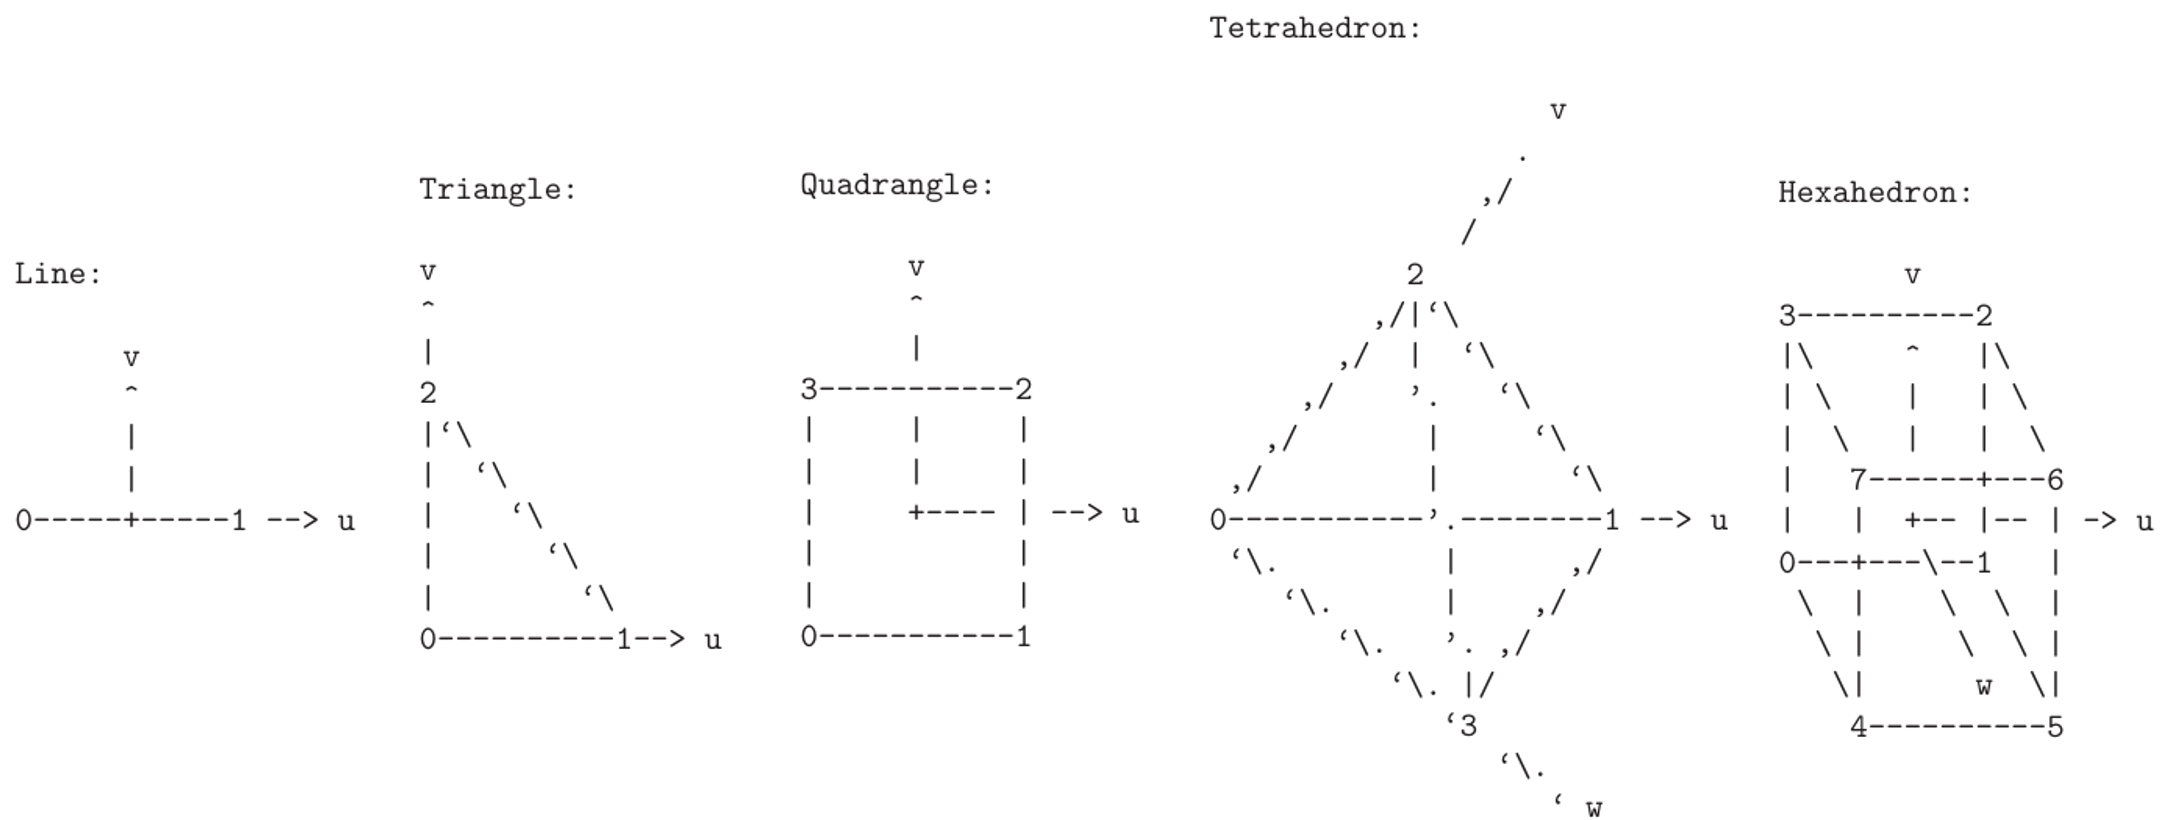
\includegraphics[width=18cm]{./pic/fig1.png}
\end{center}
\end{figure}

\section{Gmsh application programming interface}
The Gmsh application programming interface (API) allows to integrate the Gmsh library in external applications written in Python. By design, the Gmsh API is purely functional, and only uses elementary types from the target languages. See the tutorials/python directories. For other API examples, see the examples/api directory.\par
The structure of the API reflects the underlying Gmsh data model.
\begin{itemize}
\item There are two main data containers: models (which hold the geometrical and the mesh data) and views (which hold post-processing data). These are manipulated by the API functions in the top-level namespaces gmsh/model and gmsh/view, respectively. The other top-level namespaces are gmsh/option (which handles all options), gmsh/plugin (which handles extensions to core Gmsh functionality), gmsh/graphics (which handles drawing), gmsh/fltk (which handles the graphical user interface), gmsh/parser (which handles the Gmsh parser), gmsh/onelab (which handles ONELAB parameters and communications with external codes) and gmsh/logger (which handles information logging).
\item Geometrical data is made of model entities, called points (entities of dimension 0), curves (entities of dimension 1), surfaces (entities of dimension 2) or volumes (entities of dimension 3). Model entities are stored using a boundary representation: a volume is bounded by a set of surfaces, a surface is bounded by a series of curves, and a curve is bounded by two end points. Volumes and surfaces can also store embedded entities of lower dimension, to force a subsequent mesh to be conformal to internal features like a point in the middle of
a surface. Model entities are identified by a pair of integers: their dimension dim (0, 1, 2 or 3) and their tag, a strictly positive identification number. When dealing with multiple geometrical entities of possibly different dimensions, the API packs them as a vector of (dim, tag) integer pairs. Physical groups are collections of model entities and are also identified by their dimension and by a tag. Operations which do not directly reference a model are performed on the current model.
\item Model entities can be either CAD entities (from the built-in geo kernel or from the OpenCASCADE occ kernel) or discrete entities (defined by a mesh). Operations on CAD entities are performed directly within their respective CAD kernels (i.e. using functions from the
gmsh/model/geo or gmsh/model/occ namespaces, respectively), as Gmsh does not translate across CAD formats but rather directly accesses the native representation. CAD entities must be synchronized with the model in order to be meshed, or, more generally, for functions outside of gmsh/model/geo or gmsh/model/occ to manipulate them. 1D and 2D meshing algorithms use the parametrization of the underlying geometrical curve or surface to generate the mesh. Discrete entities can be remeshed provided that a parametrization is
explicitly recomputed for them.
\item Mesh data is made of elements (points, lines, triangles, quadrangles, tetrahedra, hexahedra, prisms, pyramids, ...), defined by an ordered list of their nodes. Elements and nodes are identified by tags (strictly positive identification numbers), and are stored (classified) in the model entity they discretize. Once meshed, a model entity of dimension 0 (a geometrical point) will thus contain a mesh element of type point, as well as a mesh node. A model curve will contain line elements (e.g. of MSH type 1 or 8 for first order or second order meshes, respectively) as well as its interior nodes, while its boundary nodes will be stored in the bounding model points. A model surface will contain triangular and/or quadrangular elements and all the nodes not classified on its boundary or on its embedded entities (curves and points). A model volume will contain tetrahedra, hexahedra, etc. and all the nodes not classified on its boundary or on its embedded entities (surfaces, curves and points). This data model allows to easily and efficiently handle the creation, modification and destruction of conformal meshes. All the mesh-related functions are provided in the gmsh/model/mesh namespace.
\item Post-processing data is made of views. Each view is identified by a tag, and can also be accessed by its index (which can change when views are sorted, added or deleted). A view stores both display options and data, unless the view is an alias of another view (in which
case it only stores display options, and the data points to a reference view). View data can contain several steps (e.g. to store time series) and can be either linked to one or more models1 (mesh-based data, as stored in MSH files) or independent from any model (list-based data, as stored in parsed POS files). Various plugins exist to modify and create views.
\end{itemize}

\subsection{Namespace gmsh: top-level functions}
\begin{itemize}
\item gmsh/initialize : Initialize the Gmsh API. This must be called before any call to the other functions in the API. If argvis provided, they will be handled in the same way as the command line arguments in the Gmsh app. If readConfigFiles is set, read system Gmsh configuration files (gmshrc and gmsh options). If run is set, run in the same way as the Gmsh app, either interactively or in batch mode depending on the command line arguments. If run is not set, initializing the API sets the options "General.AbortOnError" to 2 and "General.Terminal" to 1.
\begin{itemize}
\item Input : argv = [] (command line arguments), readConfigFiles = True (boolean), run = False (boolean)
\item Return : -
\end{itemize}
\item gmsh/initializeed : Return 1 if the Gmsh API is initialized, and 0 if not.
\begin{itemize}
\item Input : -
\item Return : interger
\end{itemize}
\item gmsh/finalize : Finalize the Gmsh API. This must be called when you are done using the Gmsh API.
\begin{itemize}
\item Input : -
\item Return : -
\end{itemize}
\item gmsh/open : Open a file. Equivalent to the File-$>$Open menu in the Gmsh app. Handling of the file depends on its extension and/or its contents: opening a file with model data will create a new model.
\begin{itemize}
\item Input : fileName (string)
\item Return : -
\end{itemize}
\item gmsh/merge : Merge a file. Equivalent to the File-$>$Merge menu in the Gmsh app. Handling of the file depends on its extension and/or its contents. Merging a file with model data will add the data to the current model.
\begin{itemize}
\item Input : fileName (string)
\item Return : -
\end{itemize}
\item gmsh/write : Write a file. The export format is determined by the file extension.
\begin{itemize}
\item Input : fileName (string)
\item Return : -
\end{itemize}
\item gmsh/clear : Clear all loaded models and post-processing data, and add a new empty model.
\begin{itemize}
\item Input : -
\item Return : -
\end{itemize}
\end{itemize}

\subsection{Namespace gmsh/model: model functions}
\begin{itemize}
\item gmsh/model/add : Add a new model, with name, and set it as the current model.
\begin{itemize}
\item Input : name (string)
\item Return : -
\end{itemize}
\item gmsh/model/remove : Remove the current model.
\begin{itemize}
\item Input : -
\item Return : -
\end{itemize}
\item gmsh/model/list : List the names of all models.
\begin{itemize}
\item Input : -
\item Return : names (vector of string)
\end{itemize}
\item gmsh/model/getCurrent : Get the name of the current model.
\begin{itemize}
\item Input : -
\item Return : name (string)
\end{itemize}
\item gmsh/model/setCurrent : Set the current model to the model with name. If several models have the same name, select the one that was added first.
\begin{itemize}
\item Input : name (string)
\item Return : -
\end{itemize}
\item gmsh/model/getFileName : Get the file name (if any) associated with the current model. A file name is associated when a model is read from a file on disk.
\begin{itemize}
\item Input : fileName (string)
\item Return : -
\end{itemize}
\item gmsh/model/setFileName : Set the file name associated with the current model.
\begin{itemize}
\item Input : fileName (string)
\item Return : -
\end{itemize}
\item gmsh/model/getEntities : Get all the entities in the current model. A model entity is represented by two integers: its dimension (dim == 0, 1, 2 or 3) and its tag (its unique, strictly positive identifier). If dim is $>$= 0, return only the entities of the specified dimension (e.g. points if dim == 0). The entities are returned as a vector of (dim, tag) pairs
\begin{itemize}
\item Input : dim = -1 (interger)
\item Return : dimTags (vector of pairs of integers)
\end{itemize}
\item gmsh/model/setEntityName : Set the name of the entity of dimension and tag.
\begin{itemize}
\item Input : dim (integer), tag (integer), name (string)
\item Return : -
\end{itemize}
\item gmsh/model/getEntityName : Get the name of the entity of dimension and tag.
\begin{itemize}
\item Input : dim (integer), tag (integer)
\item Return : name (string)
\end{itemize}
\item gmsh/model/removeEntityName : Remove the entity name from the current model.
\begin{itemize}
\item Input : name (string)
\item Return : -
\end{itemize}
\item gmsh/model/getPhysicalGroups : Get all the physical groups in the current model. If dim is $>$= 0, return only the entities of the specified dimension (e.g. physical points if dim == 0). The entities are returned as a vector of (dim, tag) pairs.
\begin{itemize}
\item Input : dim = -1 (integer)
\item Return : dimTags (vector of pairs of integers)
\end{itemize}
\item gmsh/model/getEntitiesForPhysicalGroup : Get the tags of the model entities making up the physical group of dimension and tag.
\begin{itemize}
\item Input : dim (integer), tag (integer)
\item Return : tags (vector of integers)
\end{itemize}
\item gmsh/model/getEntitiesForPhysicalName : Get the model entities (as a vector (dim, tag) pairs) making up the physical group
with name name.
\begin{itemize}
\item Input : name (string)
\item Return : dimTags (vector of pairs of integers)
\end{itemize}
\item gmsh/model/getPhysicalGroupsForEntity : Get the tags of the physical groups (if any) to which the model entity of dimension dim and tag tag belongs.
\begin{itemize}
\item Input : dim (integer), tag (integer)
\item Return : physicalTags (vector of integers)
\end{itemize}
\item gmsh/model/addPhysicalGroup : Add a physical group of dimension, grouping the model entities with tags. Return the tag of the physical group, equal to tag if tag is positive, or a new tag if tag $<$ 0. Set the name of the physical group if name is not empty.
\begin{itemize}
\item Input : dim (integer), tags (vector of integers), tag = -1 (integer), name = "" (string)
\item Return : integer
\end{itemize}
\item gmsh/model/removePhysicalGroups : Remove the physical groups dimTags (given as a vector of (dim, tag) pairs) from the current model. If dimTags is empty, remove all groups.
\begin{itemize}
\item Input : dimTags = [] (vector of pairs of integers)
\item Return : -
\end{itemize}
\item gmsh/model/setPhysicalName : Set the name of the physical group of dimension and tag.
\begin{itemize}
\item Input : dim (integer), tag (integer), name (string)
\item Return : -
\end{itemize}
\item gmsh/model/getPhysicalName : Get the name of the physical group of dimension and tag.
\begin{itemize}
\item Input : dim (integer), tag (integer)
\item Return : name (string)
\end{itemize}
\item gmsh/model/removePhysicalName : Remove the physical name name from the current model.
\begin{itemize}
\item Input : name (string)
\item Return : -
\end{itemize}
\item gmsh/model/setTag : Set the tag of the entity of dimension and tag to the new value.
\begin{itemize}
\item Input : dim (integer), tag (integer), newTag (integer)
\item Return : -
\end{itemize}
\item gmsh/model/getBoundary : Get the boundary of the model entities dimTags, given as a vector of (dim, tag) pairs. Return in outDimTags the boundary of the individual entities (if combined is false) or the boundary of the combined geometrical shape formed by all input entities (if combined is true). Return tags multiplied by the sign of the boundary entity if oriented is true. Apply the boundary operator recursively down to dimension 0 (i.e. to points) if recursive is true.
\begin{itemize}
\item Input : dimTags (vector of pairs of integers), combined = True (boolean), oriented = True (boolean), recursive = False (boolean)
\item Return : outDimTags (vector of pairs of integers)
\end{itemize}
\item gmsh/model/getAdjacencies : Get the upward and downward adjacencies of the model entity of dimension and tag. The upward vector returns the tags of adjacent entities of dimension dim + 1; the downward vector returns the tags of adjacent entities of dimension dim - 1.
\begin{itemize}
\item Input : dim (integer), tag (integer)
\item Return : upward (vector of integers), downward (vector of integers)
\end{itemize}
\item gmsh/model/getEntitiesInBoundingBox : Get the model entities in the bounding box defined by the two points (xmin, ymin, zmin) and (xmax, ymax, zmax). If dim is $>$= 0, return only the entities of the specified dimension (e.g. points if dim == 0).
\begin{itemize}
\item Input : xmin (double), ymin (double), zmin (double), xmax (double), ymax (double), zmax (double), dim = -1 (integer)
\item Return : dimTags (vector of pairs of integers)
\end{itemize}
\item gmsh/model/getDimension : Return the geometrical dimension of the current model.
\begin{itemize}
\item Input : 
\item Return : integer
\end{itemize}
\item gmsh/model/removeEntities : Remove the entities dimTags (given as a vector of (dim, tag) pairs) of the current model, provided that they are not on the boundary of (or embedded in) higher dimensional entities. If recursive is true, remove all the entities on their boundaries, down to dimension 0.
\begin{itemize}
\item Input : dimTags (vector of pairs of integers), recursive = False (boolean)
\item Return : -
\end{itemize}
\item gmsh/model/getType : Get the type of the entity of dimension dim and tag tag.
\begin{itemize}
\item Input : dim (integer), tag (integer)
\item Return : entityType (string)
\end{itemize}
\item gmsh/model/getParent : In a partitioned model, get the parent of the entity of dimension and tag, i.e. from which the entity is a part of, if any. parentDim and parentTag are set to -1 if the entity has no parent.
\begin{itemize}
\item Input : dim (integer), tag (integer)
\item Return : parentDim (integer), parentTag (integer)
\end{itemize}
\item gmsh/model/getNormal : Get the normal to the surface with tag tag at the parametric coordinates parametricCoord. The parametricCoord vector should contain u and v coordinates, concatenated: [p1u, p1v, p2u, ...]. normals are returned as a vector of x, y, z components, concatenated: [n1x, n1y, n1z, n2x, ...].
\begin{itemize}
\item Input : tag (integer), parametricCoord (vector of doubles)
\item Return : normals (vector of doubles)
\end{itemize}
\item gmsh/model/getParametrization : Get the parametric coordinates parametricCoord for the points coord on the entity of dimension dim and tag tag. coord are given as x, y, z coordinates, concatenated: [p1x, p1y, p1z, p2x, ...]. parametricCoord returns the parametric coordinates t on the curve (if dim = 1) or u and v coordinates concatenated on the surface (if dim == 2), i.e. [p1t, p2t, ...] or [p1u, p1v, p2u, ...].
\begin{itemize}
\item Input : dim (integer), tag (integer), coord (vector of doubles)
\item Return : parametricCoord (vector of doubles)
\end{itemize}
\item gmsh/model/isInside : Check if the coordinates (or the parametric coordinates if parametric is set) provided in coord correspond to points inside the entity of dimension dim and tag tag, and return the number of points inside. This feature is only available for a subset of entities, depending on the underlying geometrical representation.
\begin{itemize}
\item Input : dim (integer), tag (integer), coord (vector of doubles), parametric = False (boolean)
\item Return : -
\end{itemize}
\item gmsh/model/getClosestPoint : Get the points closestCoord on the entity of dimension dim and tag tag to the points coord, by orthogonal projection. coord and closestCoord are given as x, y, z coordinates, concatenated: [p1x, p1y, p1z, p2x, ...]. parametricCoord returns the parametric coordinates t on the curve (if dim == 1) or u and v coordinates concatenated on the surface (if dim = 2), i.e. [p1t, p2t, ...] or [p1u, p1v, p2u, ...].
\begin{itemize}
\item Input : dim (integer), tag (integer), coord (vector of doubles)
\item Return : closestCoord (vector of doubles), parametricCoord (vector of doubles)
\end{itemize}
\item gmsh/model/setCoordinates : Set the x, y, z coordinates of a geometrical point.
\begin{itemize}
\item Input : tag (integer), x (double), y (double), z (double)
\item Return : -
\end{itemize}
\end{itemize}

\subsection{Namespace gmsh/model/mesh: mesh functions}
\begin{itemize}
\item gmsh/model/mesh/generate : Generate a mesh of the current model, up to dimension dim (0, 1, 2 or 3).
\begin{itemize}
\item Input : dim = 3 (integer)
\item Return : -
\end{itemize}
\item gmsh/model/mesh/optimize : Optimize the mesh of the current model using method (empty for default tetrahedral mesh optimizer, "Netgen" for Netgen optimizer, "HighOrder" for direct high-order mesh optimizer, "HighOrderElastic" for high-order elastic smoother, "HighOrder FastCurving" for fast curving algorithm, "Laplace2D" for Laplace smoothing, "Relocate2D" and "Relocate3D" for node relocation, "QuadQuasiStructured" for quad mesh optimization, "UntangleMeshGeometry" for untangling). If force is set apply the optimization also to discrete entities. If dimTags (given as a vector of (dim, tag) pairs) is given, only apply the optimizer to the given entities.
\begin{itemize}
\item Input : method = "" (string), force = False (boolean), niter = 1 (integer), dimTags = [] (vector of pairs of integers)
\item Return : -
\end{itemize}
\item gmsh/model/mesh/recombine : Recombine the mesh of the current model.
\begin{itemize}
\item Input : -
\item Return : -
\end{itemize}
\item gmsh/model/mesh/refine : Refine the mesh of the current model by uniformly splitting the elements.
\begin{itemize}
\item Input : -
\item Return : -
\end{itemize}
\item gmsh/model/mesh/clear : Clear the mesh, i.e. delete all the nodes and elements, for the entities dimTags, given as a vector of (dim, tag) pairs. If dimTags is empty, clear the whole mesh. Note that the mesh of an entity can only be cleared if this entity is not on the boundary of another entity with a non-empty mesh.
\begin{itemize}
\item Input : dimTags = [] (vector of pairs of integers)
\item Return : -
\end{itemize}
\item gmsh/model/mesh/getNodes : Get the nodes classified on the entity of dimension and tag. If tag $<$ 0, get the nodes for all entities of dimension dim. If dim and tag are negative, get all the nodes in the mesh. nodeTags contains the node tags (their unique, strictly positive
identification numbers). coord is a vector of length 3 times the length of nodeTags that contains the x, y, z coordinates of the nodes, concatenated: [n1x, n1y, n1z, n2x,...]. If dim >= 0 and returnParamtricCoord is set, parametricCoord contains the parametric coordinates ([u1, u2, ...] or [u1, v1, u2, ...]) of the nodes, if available. The length of parametricCoord can be 0 or dim times the length of nodeTags. If includeBoundary is set, also return the nodes classified on the boundary of the entity (which will be reparametrized on the entity if dim $>$= 0 in order to compute their parametric coordinates).
\begin{itemize}
\item Input : dim = -1 (integer), tag = -1 (integer), includeBoundary = False (boolean), returnParametricCoord = True (boolean)
\item Return : nodeTags (vector of sizes), coord (vector of doubles), parametricCoord (vector of doubles)
\end{itemize}
\item gmsh/model/mesh/getNode : Get the coordinates and the parametric coordinates (if any) of the node with tag , as well as the dimension dim and tag tag of the entity on which the node is classified. This function relies on an internal cache (a vector in case of dense
node numbering, a map otherwise); for large meshes accessing nodes in bulk is often preferable.
\begin{itemize}
\item Input : nodeTag (size)
\item Return : coord (vector of doubles), parametricCoord (vector of doubles), dim (integer), tag (integer)
\end{itemize}
\item gmsh/model/mesh/getNodesForPhysicalGroup : Get the nodes from all the elements belonging to the physical group of dimension and tag. nodeTags contains the node tags; coord is a vector of length 3 times the length of nodeTags that contains the x, y, z coordinates of the nodes, concatenated: [n1x, n1y, n1z, n2x, ...].
\begin{itemize}
\item Input : dim (integer), tag (integer)
\item Return : nodeTags (vector of sizes), coord (vector of doubles)
\end{itemize}
\item gmsh/model/mesh/getElements : Get the elements classified on the entity of dimension dim and tag tag. If tag $<$ 0, get the elements for all entities of dimension dim. If dim and tag are negative, get all the elements in the mesh. elementTypes contains the MSH types of the elements (e.g. 2 for 3-node triangles: see getElementProperties to obtain the properties for a given element type). elementTags is a vector of the same length as elementTypes; each entry is a vector containing the tags (unique, strictly positive identifiers) of the elements of the corresponding type. nodeTags is also a vector of the same length as elementTypes; each entry is a vector of length equal to the number of elements of the given type times the number N of nodes for this type of element, that contains
the node tags of all the elements of the given type, concatenated: [e1n1, e1n2, ..., e1nN, e2n1, ...].
\begin{itemize}
\item Input : dim = -1 (integer), tag = -1 (integer)
\item Return : elementTypes (vector of integers), elementTags (vector of vectors of sizes), nodeTags (vector of vectors of sizes)
\end{itemize}
\item gmsh/model/mesh/getElement : Get the type and node tags of the element with tag tag, as well as the dimension dim and tag tag of the entity on which the element is classified. This function relies on an internal cache (a vector in case of dense element numbering, a map otherwise); for large meshes accessing elements in bulk is often preferable.
\begin{itemize}
\item Input : elementTag (size)
\item Return : elementType (integer), nodeTags (vector of sizes), dim (integer), tag (integer)
\end{itemize}
\item gmsh/model/mesh/getIntegrationPoints : Get the numerical quadrature information for the given element type elementType and integration rule integrationType, where integrationType concatenates the integration rule family name with the desired order (e.g. "Gauss4" for a quadrature suited for integrating 4th order polynomials). The "CompositeGauss" family uses tensor-product rules based the 1D Gauss-Legendre rule; the "Gauss" family uses an economic scheme when available (i.e. with a minimal number of points), and falls
back to "CompositeGauss" otherwise. Note that integration points for the "Gauss" family can fall outside of the reference element for high-order rules. localCoord contains the u, v, w coordinates of the G integration points in the reference element: [g1u, g1v, g1w, ..., gGu, gGv, gGw]. weights contains the associated weights: [g1q,..., gGq].
\begin{itemize}
\item Input : elementType (integer), integrationType (string)
\item Return : localCoord (vector of doubles), weights (vector of doubles)
\end{itemize}
\item gmsh/model/mesh/getBasisFunctions : Get the basis functions of the element of type elementType at the evaluation points localCoord (given as concatenated u, v, w coordinates in the reference element [g1u, g1v, g1w, ..., gGu, gGv, gGw]), for the function space functionSpaceType. Currently supported function spaces include "Lagrange" and "GradLagrange" for isoparametric Lagrange basis functions and their gradient in the u, v, w coordinates of the reference element; "LagrangeN" and "GradLagrangeN", with N = 1, 2, ...,
for N-th order Lagrange basis functions; "H1LegendreN" and "GradH1LegendreN", with N = 1, 2, ..., for N-th order hierarchical H1 Legendre functions; "HcurlLegendreN" and "CurlHcurlLegendreN", with N = 1, 2, ..., for N-th order curl-conforming basis functions. numComponents returns the number C of components of a basis function (e.g. 1 for scalar functions and 3 for vector functions). basisFunctions returns the value of the N basis functions at the evaluation points, i.e. [g1f1, g1f2, ..., g1fN, g2f1, ...] when C == 1 or [g1f1u, g1f1v, g1f1w, g1f2u, ..., g1fNw, g2f1u, ...] when C == 3. For basis functions that depend on the orientation of the elements, all values for the first orientation are returned first, followed by values for the second, etc. numOrientations returns the overall number of orientations. If
the wantedOrientations vector is not empty, only return the values for the desired orientation indices.
\begin{itemize}
\item Input : elementType (integer), localCoord (vector of doubles), functionSpaceType (string), wantedOrientations = [] (vector of integers)
\item Return : numComponents (integer), basisFunctions (vector of doubles), numOrientations (integer)
\end{itemize}
\item gmsh/model/mesh/getBasisFunctionsOrientation : Get the orientation index of the elements of type elementType in the entity of tag tag. The arguments have the same meaning as in getBasisFunctions. basisFunctionsOrientation is a vector giving for each element the orientation index in the values returned by getBasisFunctions. For Lagrange basis functions the call is superfluous as it will return a vector of zeros. If numTasks $>$ 1, only compute and return the part of the data indexed by task (for C++ only; output vector must be preallocated).
\begin{itemize}
\item Input : elementType (integer), functionSpaceType (string), tag = -1 (integer), task = 0 (size), numTasks = 1 (size)
\item Return : basisFunctionsOrientation (vector of integers)
\end{itemize}
\item gmsh/model/mesh/getBasisFunctionsOrientationForElement : Get the orientation of a single element elementTag.
\begin{itemize}
\item Input : elementTag (size), functionSpaceType (string)
\item Return : basisFunctionsOrientation (integer)
\end{itemize}
\item gmsh/model/mesh/getEdges : Get the global unique mesh edge identifiers edgeTags and orientations edgeOrientation for an input list of node tag pairs defining these edges, concatenated in the vector nodeTags. Mesh edges are created e.g. by createEdges(), getKeys() or addEdges(). The reference positive orientation is n1 $<$ n2, where n1 and n2 are the tags of the two edge nodes, which corresponds to
the local orientation of edge-based basis functions as well.
\begin{itemize}
\item Input : nodeTags (vector of sizes)
\item Return : edgeTags (vector of sizes), edgeOrientations (vector of integers)
\end{itemize}
\item gmsh/model/mesh/getFaces : Get the global unique mesh face identifiers faceTags and orientations faceOrientations for an input list of a multiple of three (if faceType == 3) or four (if faceType == 4) node tags defining these faces, concatenated in the vector nodeTags. Mesh faces are created e.g. by createFaces(), getKeys() or addFaces().
\begin{itemize}
\item Input : faceType (integer), nodeTags (vector of sizes)
\item Return : faceTags (vector of sizes), faceOrientations (vector of integers)
\end{itemize}
\item gmsh/model/mesh/createEdges : Create unique mesh edges for the entities dimTags, given as a vector of (dim, tag) pairs.
\begin{itemize}
\item Input : dimTags = [] (vector of pairs of integers)
\item Return : -
\end{itemize}
\item gmsh/model/mesh/createFaces : Create unique mesh faces for the entities dimTags, given as a vector of (dim, tag)
\begin{itemize}
\item Input : dimTags = [] (vector of pairs of integers)
\item Return : -
\end{itemize}
\item gmsh/model/mesh/getAllEdges : Get the global unique identifiers edgeTags and the nodes edgeNodes of the edges in the mesh. Mesh edges are created e.g. by createEdges(), getKeys() or addEdges().
\begin{itemize}
\item Input : -
\item Return : edgeTags (vector of sizes), edgeNodes (vector of sizes)
\end{itemize}
\item gmsh/model/mesh/getAllFaces : Get the global unique identifiers faceTags and the nodes faceNodes of the faces of type faceType in the mesh. Mesh faces are created e.g. by createFaces(), getKeys() or addFaces().
\begin{itemize}
\item Input : faceType (integer)
\item Return : faceTags (vector of sizes), faceNodes (vector of sizes)
\end{itemize}
\item gmsh/model/mesh/addEdges : Add mesh edges defined by their global unique identifiers edgeTags and their nodes edgeNodes.
\begin{itemize}
\item Input : edgeTags (vector of sizes), edgeNodes (vector of sizes)
\item Return : -
\end{itemize}
\item gmsh/model/mesh/addFaces : Add mesh faces of type faceType defined by their global unique identifiers faceTags and their nodes faceNodes.
\begin{itemize}
\item Input : faceType (integer), faceTags (vector of sizes), faceNodes (vector of sizes)
\item Return : -
\end{itemize}
\item gmsh/model/mesh/importStl : Import the model STL representation (if available) as the current mesh.
\begin{itemize}
\item Input : -
\item Return : -
\end{itemize}
\item gmsh/model/mesh/getDuplicateNodes : Get the tags of any duplicate nodes in the mesh of the entities dimTags, given as a vector of (dim, tag) pairs. If dimTags is empty, consider the whole mesh.
\begin{itemize}
\item Input : dimTags = [] (vector of pairs of integers)
\item Return : tags (vector of sizes)
\end{itemize}
\item gmsh/model/mesh/removeDuplicateNodes : Remove duplicate nodes in the mesh of the entities dimTags, given as a vector of (dim, tag) pairs. If dimTags is empty, consider the whole mesh.
\begin{itemize}
\item Input : dimTags = [] (vector of pairs of integers)
\item Return : -
\end{itemize}
\item gmsh/model/mesh/removeDuplicateElements : Remove duplicate elements (defined by the same nodes, in the same entity) in the
mesh of the entities dimTags, given as a vector of (dim, tag) pairs. If dimTags is
empty, consider the whole mesh.
\begin{itemize}
\item Input : dimTags = [] (vector of pairs of integers)
\item Return : -
\end{itemize}
\item gmsh/model/mesh/splitQuadrangles : Split (into two triangles) all quadrangles in surface tag whose quality is lower than quality. If tag $<$ 0, split quadrangles in all surfaces.
\begin{itemize}
\item Input : quality = 1. (double), tag = -1 (integer)
\item Return : -
\end{itemize}
\item gmsh/model/mesh/createGeometry : Create a geometry for the discrete entities dimTags (given as a vector of (dim, tag) pairs) represented solely by a mesh (without an underlying CAD description), i.e. create a parametrization for discrete curves and surfaces, assuming that each can be parametrized with a single map. If dimTags is empty, create a geometry for all the discrete entities.
\begin{itemize}
\item Input : dimTags = [] (vector of pairs of integers)
\item Return : -
\end{itemize}
\item gmsh/model/mesh/createTopology : Create a boundary representation from the mesh if the model does not have one (e.g. when imported from mesh file formats with no BRep representation of the underlying model). If makeSimplyConnected is set, enforce simply connected discrete surfaces and volumes. If exportDiscrete is set, clear any built-in CAD kernel entities and export the discrete entities in the built-in CAD kernel.
\begin{itemize}
\item Input : makeSimplyConnected = True (boolean), exportDiscrete = True (boolean)
\item Return : -
\end{itemize}
\end{itemize}

\subsection{Namespace gmsh/model/geo: built-in CAD kernel functions}
\begin{itemize}
\item gmsh/model/geo/addPoint : Add a geometrical point in the built-in CAD representation, at coordinates (x, y, z). If meshSize is $>$ 0, add a meshing constraint at that point. If tag is positive, set the tag explicitly; otherwise a new tag is selected automatically. Return the tag of the point. (Note that the point will be added in the current model only after synchronize is called. This behavior holds for all the entities added in the geo module.)
\begin{itemize}
\item Input : x (double), y (double), z (double), meshSize = 0. (double), tag = -1 (integer)
\item Return : -
\end{itemize}
\item gmsh/model/geo/addLine : Add a straight line segment in the built-in CAD representation, between the two points with tags startTag and endTag. If tag is positive, set the tag explicitly; otherwise a new tag is selected automatically. Return the tag of the line.
\begin{itemize}
\item Input : startTag (integer), endTag (integer), tag = -1 (integer)
\item Return : -
\end{itemize}
\item gmsh/model/geo/addCurveLoop : Add a curve loop (a closed wire) in the built-in CAD representation, formed by the curves curveTags. curveTags should contain (signed) tags of model entities of dimension 1 forming a closed loop: a negative tag signifies that the underlying curve is considered with reversed orientation. If tag is positive, set the tag explicitly; otherwise a new tag is selected automatically. If reorient is set, automatically reorient the curves if necessary. Return the tag of the curve loop.
\begin{itemize}
\item Input : curveTags (vector of integers), tag = -1 (integer), reorient = False (boolean)
\item Return : -
\end{itemize}
\item gmsh/model/geo/addSurfaceFilling : Add a surface in the built-in CAD representation, filling the curve loops in wireTags using transfinite interpolation. Currently only a single curve loop is supported; this curve loop should be composed by 3 or 4 curves only. If tag is positive, set the tag explicitly; otherwise a new tag is selected automatically. Return the tag of the surface.
\begin{itemize}
\item Input : wireTags (vector of integers), tag = -1 (integer), sphereCenterTag = -1 (integer)
\item Return : -
\end{itemize}
\item gmsh/model/geo/addSurfaceLoop : Add a surface loop (a closed shell) formed by surfaceTags in the built-in CAD representation. If tag is positive, set the tag explicitly; otherwise a new tag is selected automatically. Return the tag of the shell.
\begin{itemize}
\item Input : surfaceTags (vector of integers), tag = -1 (integer)
\item Return : -
\end{itemize}
\item gmsh/model/geo/addVolume : Add a volume (a region) in the built-in CAD representation, defined by one or more shells shellTags. The first surface loop defines the exterior boundary; additional surface loop define holes. If tag is positive, set the tag explicitly; otherwise a new tag is selected automatically. Return the tag of the volume.
\begin{itemize}
\item Input : shellTags (vector of integers), tag = -1 (integer)
\item Return : -
\end{itemize}
\item gmsh/model/geo/getMaxTag : Get the maximum tag of entities of dimension in the built-in CAD representation.
\begin{itemize}
\item Input : dim (integer)
\item Return : -
\end{itemize}
\item gmsh/model/geo/addPhysicalGroup : Add a physical group of dimension dim, grouping the entities with tags tags in the built-in CAD representation. Return the tag of the physical group, equal to tag if tag is positive, or a new tag if tag < 0. Set the name of the physical group if name is not empty.
\begin{itemize}
\item Input : dim (integer), tags (vector of integers), tag = -1 (integer), name = "" (string)
\item Return : -
\end{itemize}
\end{itemize}

\subsection{Namespace gmsh/model/geo/mesh: built-in CAD kernel meshing constraints}
\begin{itemize}
\item gmsh/model/geo/mesh/setSize : Set a mesh size constraint on the entities dimTags (given as a vector of (dim, tag) pairs) in the built-in CAD kernel representation. Currently only entities of dimension 0 (points) are handle
\begin{itemize}
\item Input : dimTags (vector of pairs of integers), size (double)
\item Return : -
\end{itemize}
\item gmsh/model/geo/mesh/setSizeFromBoundary : Force the mesh size to be extended from the boundary, or not, for the entity of
dimension dim and tag tag in the built-in CAD kernel representation. Currently only supported for dim == 2.
\begin{itemize}
\item Input : dim (integer), tag (integer), val (integer)
\item Return : -
\end{itemize}
\end{itemize}
\end{document}










































































\section{Gmsh graphical user interface}
Once you have the Gmsh application installed, to launch the graphical interface just double-click on the Gmsh icon, or type
\begin{lstlisting}
gmsh
\end{lstlisting}
at the shell prompt in a terminal. This will open the main window of the Gmsh GUI, with a menu bar on top, a tree menu on the left (which by default contains a 'Modules' entry with three children: 'Geometry', 'Mesh' and 'Solver'), a graphic area on the right, and a status bar
with some shortcut buttons at the bottom.\par
To create a new geometrical model, use the 'File-$>$New' menu to create a new model file, and choose for example 'mymodel.geo' as file name. Then in the tree menu, successively open the 'Geometry', 'Elementary entities' and 'Add' submenus, and click for example on 'Rectangle'. A context window with parameters will pop up: you can enter some parameters in this window (e.g. the width and height of the rectangle) and move the mouse to place it on the canvas. If you don't want to place the rectangle with the mouse, select 'X', 'Y' and 'Z freeze' in the window and enter the coordinates manually in the context window. Once you are done, either press e (see the status message on the top of the graphic window) or click on the 'Add' button in the context window. \par
There is no need to save your geometrical model: when the rectangle was added, scripting commands were automatically appended to your model file 'mymodel.geo':
\begin{lstlisting}
//+
SetFactory("OpenCASCADE");
Rectangle(1) = {0, 0, 0, 1, 0.5, 0};
\end{lstlisting}
You can edit this script with any text editor; clicking on 'Edit script' in the tree menu will launch the default text editor specified by the General.Editor option. If you edit the script, you should click on 'Reload script' in the tree menu to reload the modifications in the GUI. The //+ line in the script is a comment that is used as a placemark between commands added by the GUI.\par
Combining GUI actions and script file editing is a classical way of working with the Gmsh app. For example, it is often faster to define variables and points directly in the script file, and then use the GUI to define the curves, the surfaces and the volumes interactively.\par
To load an existing model instead of creating a model from scratch, use the 'File-$>$Open' menu. For example, to open the first tutorial, choose t1.geo. On the terminal, you can also specify the file name directly on the command line, i.e.:
\begin{lstlisting}
gmsh t1.geo
\end{lstlisting}
To generate a mesh, open 'Mesh' in the tree menu and choose the desired dimension: '1D' will mesh all the curves; '2D' will mesh all the surfaces—as well as all the curves if '1D' was not called before; '3D' will mesh all the volumes—and all the surfaces if '2D' was not called
before. To save the resulting mesh in the current mesh format click on 'Save' in the tree menu, or select the appropriate format and file name with the 'File-$>$Export' menu. The default mesh file name is based on the name of the current active model, with an appended extension depending on the mesh format. Note that most interactive commands have keyboard shortcuts, or select 'Help-$>$Keyboard and Mouse Usage' in the menu. For example, to quickly generate the 2D mesh and save a mesh, you can first press2, then Ctrl+Shift+s.\par
A double-click in the graphic window will pop up a quick shortcut menu, which can be used e.g. to quickly toggle the visibility of mesh entities (like surface faces), reset the viewport, select the rotation center, display axes, or access the full module options (from the 'Tools-$>$Option' menu). The shortcut buttons on the bottom left of the status bar can be used to quickly adjust the viewport: 'X', 'Y', 'Z' set viewports with the corresponding axis perpendicular to graphic plane; the rotation button rotates the view by 90 degrees; and '1:1' resets the scale.\par
Several files can be loaded simultaneously. When specified on the command line, the first one defines the active model (in the same way as using the 'File-$>$Open' menu) and the others are 'merged' into this model (in the same way as using the the 'File-$>$Merge' menu). For example, to merge the post-processing views contained in the files view1.pos and view5.msh together, you can type the following command:
\begin{lstlisting}
gmsh t1.geo view1.pos view5.msh
\end{lstlisting}
When one or more more post-processing views are loaded, a 'Post-Processing' entry in the tree menu appears. With the previous command, three views will appear in the tree menu under 'Post-processing', respectively labeled 'A scalar map', 'Nodal scalar map' and 'Element 1 vector'. In this example the views contain several time steps: you can loop through them with the shortcuts icons on the left of the status bar. A mouse click on the view name will toggle the visibility of the selected view, while a click on the arrow button on the right will provide access to the view's options.\par
Note that all the options specified interactively can also be directly specified in the script files. You can save the current options of the current active model with the 'File-$>$Save Model Options'. This will create a new option file with the same filename as the active model, but with an extra '.opt' extension added. The next time you open this model, the associated options will be automatically loaded, too. To save the current options as your default preferences for all future Gmsh sessions, use the 'File-$>$Save Options As Default' menu instead. You can also save the current options in an arbitrary file by choosing the 'Gmsh options' format in 'File-$>$Export'. A full list of options with their current values is also available using the 'Help-$>$Current Options' menu.

\section{Gmsh command-line interface}
Gmsh defines a number of commands-line switches that can be used to control Gmsh in 'batch' mode from the command line, and pass options without resorting to a script or the API.\par
For example, meshing the first tutorial in batch mode can be done in a terminal by passing the -2 command-line switch:
\begin{lstlisting}
gmsh t1.geo -2
\end{lstlisting}
The same effect could be achieved by adding the Mesh 2; command at the end of 't1.geo' and running
\begin{lstlisting}
gmsh t1.geo -parse_and_exit
\end{lstlisting}
or further adding the Exit; command at the end of the script and simply opening this new file:
\begin{lstlisting}
gmsh t1.geo
\end{lstlisting}
Note that all numeric and string options can be set from the command line with the -setnumber and -setstring switches
\begin{lstlisting}
gmsh t1.geo -setnumber Mesh.Nodes 1 -setnumber Geometry.SurfaceLabels 1
\end{lstlisting}
The list of all command-line switches is given hereafter(Related option names, if any, are given between parentheses).
\begin{itemize}
\item Geometry
\begin{itemize}
\item -0 : Output model, then exit
\item -tol value : Set geometrical tolerance (Geometry.Tolerance)
\item -match : Match geometries and meshes
\end{itemize}
\item Mesh
\begin{itemize}
\item -1, -2, -3 : Perform 1D, 2D or 3D mesh generation, then exit
\item -format string : Select output mesh format: auto, msh1, msh2, msh22, msh3, msh4, msh40, msh41, msh, unv, vtk, wrl, mail, stl, p3d, mesh, bdf, cgns, med, diff, ir3, inp, ply2, celum, su2, x3d, dat, neu, m, key, off, rad (Mesh.Format)
\item -bin : Create binary files when possible (Mesh.Binary)
\item -refine : Perform uniform mesh refinement, then exit
\item -barycentric\_refine : Perform barycentric mesh refinement, then exit
\item -reclassify angle : Reclassify surface mesh, then exit
\item -reparam angle : Reparametrize surface mesh, then exit
\item -part int : Partition after batch mesh generation (Mesh.NbPartitions)
\item -part\_weight [tri,quad,tet,hex,pri,pyr,trih] int : Weight of a triangle/quad/etc.\\
during partitioning (Mesh.Partition[Tri,Quad,...]Weight)
\item -part\_split : Save mesh partitions in separate files (Mesh.PartitionSplitMeshFiles)
\item -part\_[no\_]topo : Create the partition topology (Mesh.PartitionCreateTopology)
\item -part\_[no\_]ghosts : Create ghost cells (Mesh.PartitionCreateGhostCells)
\item -part\_[no\_]physicals : Create physical groups for partitions (Mesh.PartitionCreatePhysicals)
\item -part\_topo\_pro : Save the partition topology .pro file (Mesh.PartitionTopologyFile)
\item -preserve\_numbering\_msh2 : Preserve element numbering in MSH2 format (Mesh.PreserveNumberingMsh2)
\item -save\_all : Save all elements (Mesh.SaveAll)
\item -save\_parametric : Save nodes with their parametric coordinates (Mesh.SaveParametric)
\item -save\_topology : Save model topology (Mesh.SaveTopology)
\item -algo string : Select mesh algorithm: auto, meshadapt, del2d, front2d, delquad, quadqs, initial2d, del3d, front3d, mmg3d, hxt, initial3d (Mesh.Algorithm and Mesh.Algorithm3D)
\item -smooth int : Set number of mesh smoothing steps (Mesh.Smoothing)
\item -order int : Set mesh order (Mesh.ElementOrder)
\item -optimize[\_netgen] : Optimize quality of tetrahedral elements (Mesh.Optimize[Netgen])
\item -optimize\_threshold : Optimize tetrahedral elements that have a quality less than a threshold\\ (Mesh.OptimizeThreshold)
\item -optimize\_ho : Optimize high order meshes (Mesh.HighOrderOptimize)
\item -ho\_[min,max,nlayers] : High-order optimization parameters (Mesh.HighOrderThreshold[Min,Max], \\Mesh.HighOrderNumLayers)
\item -clscale value : Set mesh element size factor (Mesh.MeshSizeFactor)
\item -clmin value : Set minimum mesh element size (Mesh.MeshSizeMin)
\item -clmax value : Set maximum mesh element size (Mesh.MeshSizeMax)
\item -clextend value : Extend mesh element sizes from boundaries (Mesh.MeshSizeExtendFromBoundary)
\item -clcurv value : Compute mesh element size from curvature, with value the target number of elements per 2*pi radians (Mesh.MeshSizeFromCurvature)
\item -aniso\_max value : Set maximum anisotropy for bamg (Mesh.AnisoMax)
\item -smooth\_ratio value : Set smoothing ration between mesh sizes at nodes of a same edge for bamg (Mesh.SmoothRatio)
\item -epslc1d value : Set accuracy of evaluation of mesh size field for 1D mesh (Mesh.LcIntegrationPrecision)
\item -swapangle value : Set the threshold angle (in degrees) between two adjacent faces below which a swap is allowed (Mesh.AllowSwapAngle)
\item -rand value : Set random perturbation factor (Mesh.RandomFactor)
\item -bgm file : Load background mesh from file
\item -check : Perform various consistency checks on mesh
\item -ignore\_periocity Ignore periodic boundaries (Mesh.IgnorePeriodicity)
\end{itemize}
\item Post-processing
\begin{itemize}
\item  -link int : Select link mode between views (PostProcessing.Link)
\item -combine : Combine views having identical names into multi-time-step views
\end{itemize}
\item Solver
\begin{itemize}
\item -listen string : Always listen to incoming connection requests (Solver.AlwaysListen) on the given socket (uses Solver.SocketName if not specified)
\item -minterpreter string : Name of Octave interpreter (Solver.OctaveInterpreter)
\item -pyinterpreter string : Name of Python interpreter (Solver.OctaveInterpreter)
\item -run : Run ONELAB solver(s)
\end{itemize}
\item Display
\begin{itemize}
\item -n : Hide all meshes and post-processing views on startup (View.Visible, Mesh.[Points,Lines,SurfaceEdges,...])
\item -nodb : Disable double buffering (General.DoubleBuffer)
\item -numsubedges : Set num of subdivisions for high order element display (Mesh.NumSubEdges)
\item -fontsize int : Specify the font size for the GUI (General.FontSize)
\item -theme string : Specify FLTK GUI theme (General.FltkTheme)
\item -display string : Specify display (General.Display)
\item -camera : Use camera mode view (General.CameraMode)
\item -stereo : OpenGL quad-buffered stereo rendering (General.Stereo)
\item -gamepad : Use gamepad controller if available
\end{itemize}
\item Other
\begin{itemize}
\item -, -parse\_and\_exit : Parse input files, then exit
\item -save : Save output file, then exit
\item -o : file Specify output file name
\item -new : Create new model before merge next file
\item -merge : Merge next files
\item -open : Open next files
\item -a, -g, -m, -s, -p : Start in automatic, geometry, mesh, solver or post-processing mode (General.InitialModule)
\item -pid : Print process id on stdout
\item -watch pattern : Pattern of files to merge as they become available (General.WatchFilePattern)
\item -bg file : Load background (image or PDF) file (General.BackgroundImageFileName)
\item -v int : Set verbosity level (General.Verbosity)
\item -string "string" : Parse command string at startup
\item -setnumber name value : Set constant, ONELAB or option number name=value
\item -setstring name value : Set constant, ONELAB or option string name=value
\item -nopopup : Don't popup dialog windows in scripts (General.NoPopup)
\item -noenv : Don't modify the environment at startup
\item -nolocale : Don't modify the locale at startup
\item -option file : Parse option file at startup
\item -convert files : Convert files into latest binary formats, then exit
\item -nt int : Set number of threads (General.NumThreads)
\item -cpu : Report CPU times for all operations
\item -version : Show version number
\item -info : Show detailed version information
\item -help : Show command line usage
\item -help\_options : Show all options
\end{itemize}
\end{itemize}





\end{document}















































































